\documentclass[letterpaper, 12pt]{article}

\usepackage{amsmath, amsthm, amssymb, dsfont, accents}
\usepackage{hyperref, subcaption, booktabs}
\usepackage{fullpage}

\usepackage{tikz, pgfplots}
\pgfplotsset{compat=newest}
\newlength{\figurewidth}
\newlength{\figureheight}

\newcommand{\argmin}{\operatornamewithlimits{arg\ min}}
\newcommand{\argmax}{\operatornamewithlimits{arg\ max}}
\newcommand{\ind}[1]{\mathds{1}_{{#1}}} 
\newcommand{\ubar}[1]{\underaccent{\bar}{#1}}

\title{Invariant Set Lane Keeping Controller Explained}
\author{Petter Nilsson \\ \href{mailto:pettni@umich.edu}{pettni@umich.edu}}

\begin{document}

\section{Model} % (fold)
\label{sec:model}

The controller is designed for the following 3-state model:

\begin{equation}
	\begin{bmatrix}
		\dot y \\
		\dot \psi \\
		\dot r
	\end{bmatrix}
	= 
	\begin{bmatrix}
		0 & u_0 & 0 \\
		0 & 0   & 1 \\
		0 & 0 & - \frac{a^2 C_{\alpha f} + b^2 C_{\alpha r}}{I_z u_0}
	\end{bmatrix} 
	\begin{bmatrix}
		y \\
		\psi \\
		r
	\end{bmatrix}
	+ 
	\begin{bmatrix}
		0 \\ 0 \\ \frac{a C_{\alpha f}}{I_z}
	\end{bmatrix}
	\delta_f
	+ \begin{bmatrix}
		0 & 1 \\
		1 & 0 \\
		0 & \frac{b C_{\alpha r} - a C_{\alpha f}}{I_z u_0}
	\end{bmatrix} 
	\begin{bmatrix}
		r_{road} \\
		v
	\end{bmatrix}
\end{equation}

and implemented on the 4-state model

\begin{equation}
	\begin{bmatrix}
		\dot y \\
		\dot r \\
		\dot \psi \\
		\dot r
	\end{bmatrix}
	= 
	\begin{bmatrix}
	0 & 1 & u_0 & 0 \\
    0 & -\frac{C_{\alpha f}+C_{\alpha r}}{m u_0}  & 0 & \frac{b C_{\alpha r}-a C_{\alpha f}}{m u_0} - u_0 \\
    0 & 0 & 0 & 1 \\
    0 & \frac{b C_{\alpha r}-a C_{\alpha f}}{I_z u_0} & 0 & - \frac{a^2   C_{\alpha f} + b^2   C_{\alpha r}}{Iz u_0}
	\end{bmatrix} 
	\begin{bmatrix}
		y \\
		v \\
		\psi \\
		r
	\end{bmatrix}
	+ 
	\begin{bmatrix}
		0 \\ \frac{C_{\alpha f}}{m} \\ 0 \\ \frac{a C_{\alpha f}}{I_z}
	\end{bmatrix}
	\delta_f
	+ \begin{bmatrix}
		0 \\
		0 \\
		1 \\
		0 
	\end{bmatrix} 
		r_{road} 
\end{equation}

% section model (end)

\section{Disturbance assumptions} % (fold)
\label{sec:assumptions}

Maximal road curvature: 
\begin{equation}
	r_{road} \in [- \alpha \frac{g}{u_0}, \alpha \frac{g}{u_0}]
\end{equation}

Modeling error due to setting $v=0$:
\begin{equation}
	v \in [-1, 1]
\end{equation}

% section assumptions (end)

\section{Specifications} % (fold)
\label{sec:specifications}

Don't exit the lane:
\begin{equation}
	\square (y \in [-0.9, 0.9])
\end{equation}

% section specifications (end)

\setlength\figurewidth{0.4\columnwidth} 
\setlength\figureheight{0.3 \columnwidth} 

\begin{figure}[h]
	\begin{center}
		% \includegraphics[width=0.4\columnwidth]{invariant}
		% This file was created by matlab2tikz v0.4.7 running on MATLAB 8.2.
% Copyright (c) 2008--2014, Nico Schlömer <nico.schloemer@gmail.com>
% All rights reserved.
% Minimal pgfplots version: 1.3
% 
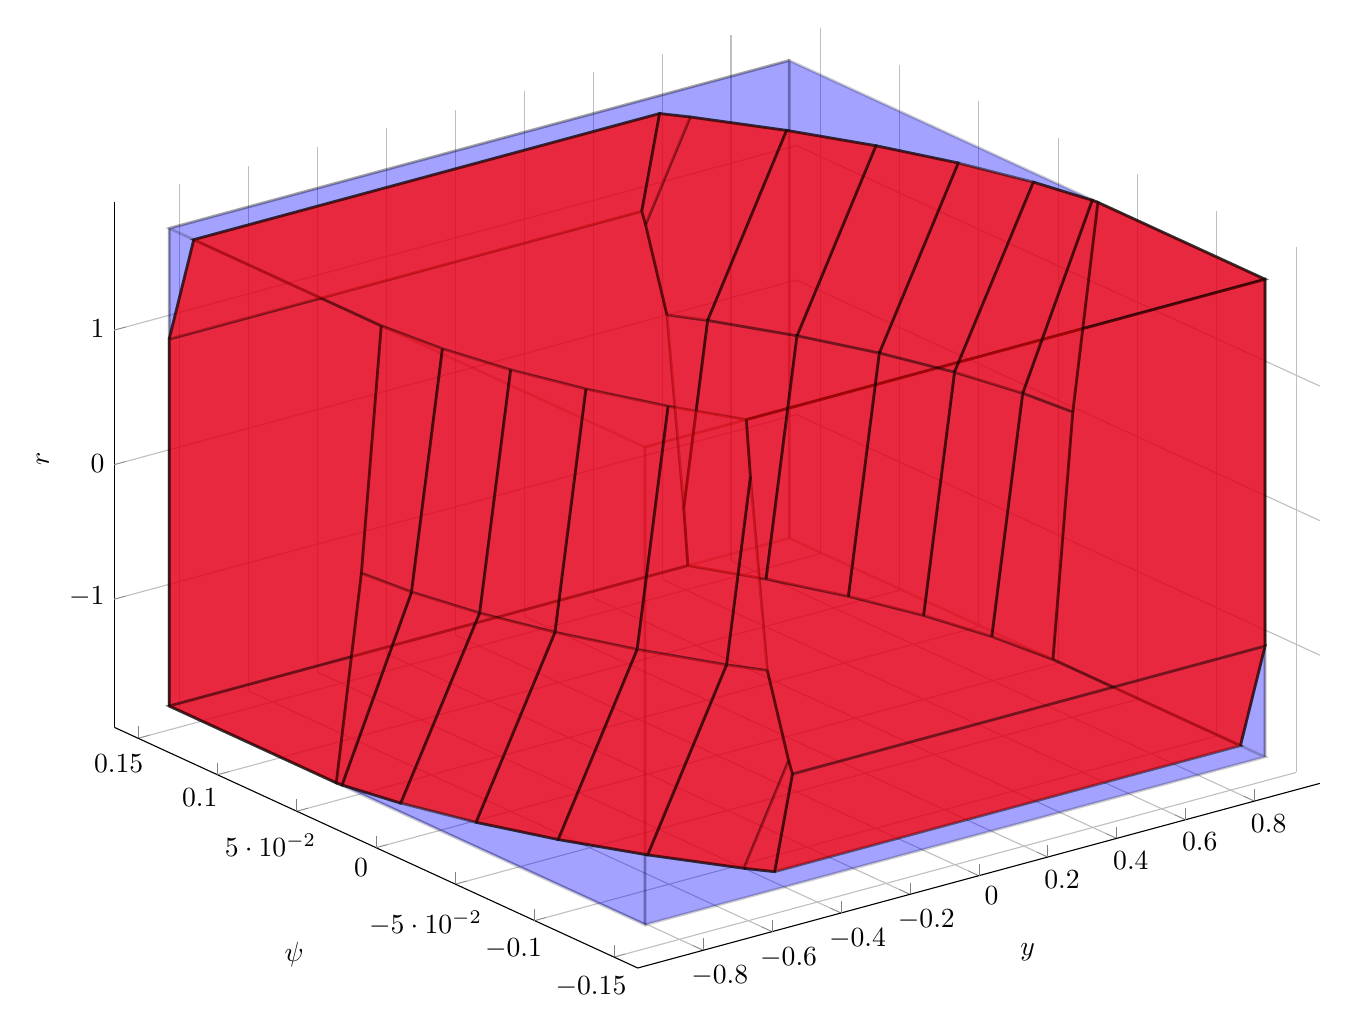
\begin{tikzpicture}

\begin{axis}[%
width=6.02777777777778in,
height=4.75416666666667in,
view={-37.5}{30},
scale only axis,
xmin=-0.99,
xmax=0.99,
xlabel={$y$},
xmajorgrids,
ymin=-0.165,
ymax=0.165,
ylabel={$\psi$},
ymajorgrids,
zmin=-1.95299910967934,
zmax=1.95299910967934,
zlabel={$r$},
zmajorgrids,
axis x line*=bottom,
axis y line*=left,
axis z line*=left
]

\addplot3[area legend,solid,line width=1.0pt,fill=blue,opacity=2.000000e-01,draw=black,forget plot]
table[row sep=crcr] {%
x	y	z\\
0.9	-0.15	-1.77545373607212\\
0.9	-0.15	1.77545373607212\\
0.9	0.15	1.77545373607212\\
0.9	0.15	-1.77545373607212\\
};


\addplot3[area legend,solid,line width=1.0pt,fill=blue,opacity=2.000000e-01,draw=black,forget plot]
table[row sep=crcr] {%
x	y	z\\
-0.9	-0.15	1.77545373607212\\
-0.9	-0.15	-1.77545373607212\\
-0.9	0.15	-1.77545373607212\\
-0.9	0.15	1.77545373607212\\
};


\addplot3[area legend,solid,line width=1.0pt,fill=blue,opacity=2.000000e-01,draw=black,forget plot]
table[row sep=crcr] {%
x	y	z\\
0.9	0.15	-1.77545373607212\\
0.9	0.15	1.77545373607212\\
-0.9	0.15	1.77545373607212\\
-0.9	0.15	-1.77545373607212\\
};


\addplot3[area legend,solid,line width=1.0pt,fill=blue,opacity=2.000000e-01,draw=black,forget plot]
table[row sep=crcr] {%
x	y	z\\
0.9	-0.15	1.77545373607212\\
-0.9	-0.15	1.77545373607212\\
-0.9	0.15	1.77545373607212\\
0.9	0.15	1.77545373607212\\
};


\addplot3[area legend,solid,line width=1.0pt,fill=blue,opacity=2.000000e-01,draw=black,forget plot]
table[row sep=crcr] {%
x	y	z\\
-0.9	-0.15	-1.77545373607212\\
-0.9	-0.15	1.77545373607212\\
0.9	-0.15	1.77545373607212\\
0.9	-0.15	-1.77545373607212\\
};


\addplot3[area legend,solid,line width=1.0pt,fill=blue,opacity=2.000000e-01,draw=black,forget plot]
table[row sep=crcr] {%
x	y	z\\
-0.9	-0.15	-1.77545373607212\\
0.9	-0.15	-1.77545373607212\\
0.9	0.15	-1.77545373607212\\
-0.9	0.15	-1.77545373607212\\
};


\addplot3[area legend,solid,line width=1.0pt,fill=red,opacity=5.000000e-01,draw=black,forget plot]
table[row sep=crcr] {%
x	y	z\\
0.9	-0.134460224004354	-1.77545373607212\\
0.9	-0.15	-0.951257668418722\\
0.9	-0.15	1.77545373607212\\
0.9	-0.0445797996829758	1.77545373607212\\
0.9	-0.0287735096778711	0.131430219551011\\
0.9	-0.0162509912512161	-1.77545373607212\\
0.9	-0.0162509912512161	-1.77545373607212\\
0.9	-0.0162509912512161	-1.77545373607212\\
0.9	-0.0162509912512161	-1.77545373607212\\
0.9	-0.0162509912512161	-1.77545373607212\\
0.9	-0.0162509912512161	-1.77545373607212\\
0.9	-0.0162509912512161	-1.77545373607212\\
0.9	-0.0162509912512161	-1.77545373607212\\
0.9	-0.0162509912512161	-1.77545373607212\\
0.9	-0.0162509912512161	-1.77545373607212\\
0.9	-0.0162509912512161	-1.77545373607212\\
};


\addplot3[area legend,solid,line width=1.0pt,fill=red,opacity=5.000000e-01,draw=black,forget plot]
table[row sep=crcr] {%
x	y	z\\
-0.9	0.0162509912512162	1.77545373607212\\
-0.9	0.0287735096778705	-0.131430219550917\\
-0.9	0.0445797996829763	-1.77545373607212\\
-0.9	0.15	-1.77545373607212\\
-0.9	0.15	0.951257668418724\\
-0.9	0.134460224004354	1.77545373607212\\
-0.9	0.134460224004354	1.77545373607212\\
-0.9	0.134460224004354	1.77545373607212\\
-0.9	0.134460224004354	1.77545373607212\\
-0.9	0.134460224004354	1.77545373607212\\
-0.9	0.134460224004354	1.77545373607212\\
-0.9	0.134460224004354	1.77545373607212\\
-0.9	0.134460224004354	1.77545373607212\\
-0.9	0.134460224004354	1.77545373607212\\
-0.9	0.134460224004354	1.77545373607212\\
-0.9	0.134460224004354	1.77545373607212\\
};


\addplot3[area legend,solid,line width=1.0pt,fill=red,opacity=5.000000e-01,draw=black,forget plot]
table[row sep=crcr] {%
x	y	z\\
0.605872399301855	0.15	-1.77545373607212\\
0.593953699501555	0.15	-1.34147400760398\\
0.544840289834663	0.15	0.131430219550891\\
0.482970432813291	0.15	0.844948729459494\\
0.471994679828053	0.15	0.951257668418724\\
-0.9	0.15	0.951257668418724\\
-0.9	0.15	-1.77545373607212\\
-0.9	0.15	-1.77545373607212\\
-0.9	0.15	-1.77545373607212\\
-0.9	0.15	-1.77545373607212\\
-0.9	0.15	-1.77545373607212\\
-0.9	0.15	-1.77545373607212\\
-0.9	0.15	-1.77545373607212\\
-0.9	0.15	-1.77545373607212\\
-0.9	0.15	-1.77545373607212\\
-0.9	0.15	-1.77545373607212\\
};


\addplot3[area legend,solid,line width=1.0pt,fill=red,opacity=5.000000e-01,draw=black,forget plot]
table[row sep=crcr] {%
x	y	z\\
0.862844026967176	-0.0120305543067136	1.77545373607212\\
0.89809687858131	-0.0414079306518254	1.77545373607212\\
0.9	-0.0445797996829758	1.77545373607212\\
0.9	-0.15	1.77545373607212\\
-0.605872399301858	-0.15	1.77545373607212\\
-0.695404353796657	-0.120156015168401	1.77545373607212\\
-0.777238648697708	-0.0860583922929626	1.77545373607212\\
-0.838614369873494	-0.0519607694175259	1.77545373607212\\
-0.879531517324016	-0.0178631465420911	1.77545373607212\\
-0.9	0.0162509912512162	1.77545373607212\\
-0.9	0.134460224004354	1.77545373607212\\
0.452168495313318	0.134460224004354	1.77545373607212\\
0.494589699912449	0.124359937195037	1.77545373607212\\
0.617341142264025	0.0902623143195997	1.77545373607212\\
0.719634010890342	0.0561646914441606	1.77545373607212\\
0.801468305791383	0.0220670685687267	1.77545373607212\\
};


\addplot3[area legend,solid,line width=1.0pt,fill=red,opacity=5.000000e-01,draw=black,forget plot]
table[row sep=crcr] {%
x	y	z\\
-0.471994679828052	-0.15	-0.951257668418722\\
-0.482970432813293	-0.15	-0.844948729459471\\
-0.544840289834663	-0.15	-0.131430219550889\\
-0.593953699501574	-0.15	1.34147400760454\\
-0.605872399301858	-0.15	1.77545373607212\\
0.9	-0.15	1.77545373607212\\
0.9	-0.15	-0.951257668418722\\
0.9	-0.15	-0.951257668418722\\
0.9	-0.15	-0.951257668418722\\
0.9	-0.15	-0.951257668418722\\
0.9	-0.15	-0.951257668418722\\
0.9	-0.15	-0.951257668418722\\
0.9	-0.15	-0.951257668418722\\
0.9	-0.15	-0.951257668418722\\
0.9	-0.15	-0.951257668418722\\
0.9	-0.15	-0.951257668418722\\
};


\addplot3[area legend,solid,line width=1.0pt,fill=red,opacity=5.000000e-01,draw=black,forget plot]
table[row sep=crcr] {%
x	y	z\\
-0.801468305791383	-0.0220670685687269	-1.77545373607212\\
-0.719634010890329	-0.0561646914441661	-1.77545373607212\\
-0.617341142264044	-0.0902623143195943	-1.77545373607212\\
-0.494589699912451	-0.124359937195037	-1.77545373607212\\
-0.452168495313317	-0.134460224004354	-1.77545373607212\\
0.9	-0.134460224004354	-1.77545373607212\\
0.9	-0.0162509912512161	-1.77545373607212\\
0.879531517324016	0.0178631465420913	-1.77545373607212\\
0.838614369873494	0.0519607694175259	-1.77545373607212\\
0.777238648697709	0.0860583922929623	-1.77545373607212\\
0.69540435379667	0.120156015168395	-1.77545373607212\\
0.605872399301855	0.15	-1.77545373607212\\
-0.9	0.15	-1.77545373607212\\
-0.9	0.0445797996829763	-1.77545373607212\\
-0.898096878581309	0.041407930651825	-1.77545373607212\\
-0.862844026967176	0.0120305543067136	-1.77545373607212\\
};


\addplot3[area legend,solid,line width=1.0pt,fill=red,opacity=5.000000e-01,draw=black,forget plot]
table[row sep=crcr] {%
x	y	z\\
0.9	-0.0287735096778711	0.131430219551011\\
0.9	-0.0445797996829758	1.77545373607212\\
0.89809687858131	-0.0414079306518254	1.77545373607212\\
0.883232162515523	-0.00082711387040806	0.131430219550865\\
0.883232162515523	-0.00082711387040806	0.131430219550865\\
0.883232162515523	-0.00082711387040806	0.131430219550865\\
0.883232162515523	-0.00082711387040806	0.131430219550865\\
0.883232162515523	-0.00082711387040806	0.131430219550865\\
0.883232162515523	-0.00082711387040806	0.131430219550865\\
0.883232162515523	-0.00082711387040806	0.131430219550865\\
0.883232162515523	-0.00082711387040806	0.131430219550865\\
0.883232162515523	-0.00082711387040806	0.131430219550865\\
0.883232162515523	-0.00082711387040806	0.131430219550865\\
0.883232162515523	-0.00082711387040806	0.131430219550865\\
0.883232162515523	-0.00082711387040806	0.131430219550865\\
0.883232162515523	-0.00082711387040806	0.131430219550865\\
};


\addplot3[area legend,solid,line width=1.0pt,fill=red,opacity=5.000000e-01,draw=black,forget plot]
table[row sep=crcr] {%
x	y	z\\
0.471994679828053	0.15	0.951257668418724\\
0.452168495313318	0.134460224004354	1.77545373607212\\
-0.9	0.134460224004354	1.77545373607212\\
-0.9	0.15	0.951257668418724\\
-0.9	0.15	0.951257668418724\\
-0.9	0.15	0.951257668418724\\
-0.9	0.15	0.951257668418724\\
-0.9	0.15	0.951257668418724\\
-0.9	0.15	0.951257668418724\\
-0.9	0.15	0.951257668418724\\
-0.9	0.15	0.951257668418724\\
-0.9	0.15	0.951257668418724\\
-0.9	0.15	0.951257668418724\\
-0.9	0.15	0.951257668418724\\
-0.9	0.15	0.951257668418724\\
-0.9	0.15	0.951257668418724\\
};


\addplot3[area legend,solid,line width=1.0pt,fill=red,opacity=5.000000e-01,draw=black,forget plot]
table[row sep=crcr] {%
x	y	z\\
0.9	-0.0162509912512161	-1.77545373607212\\
0.9	-0.0287735096778711	0.131430219551011\\
0.883232162515523	-0.00082711387040806	0.131430219550865\\
0.879531517324016	0.0178631465420913	-1.77545373607212\\
0.879531517324016	0.0178631465420913	-1.77545373607212\\
0.879531517324016	0.0178631465420913	-1.77545373607212\\
0.879531517324016	0.0178631465420913	-1.77545373607212\\
0.879531517324016	0.0178631465420913	-1.77545373607212\\
0.879531517324016	0.0178631465420913	-1.77545373607212\\
0.879531517324016	0.0178631465420913	-1.77545373607212\\
0.879531517324016	0.0178631465420913	-1.77545373607212\\
0.879531517324016	0.0178631465420913	-1.77545373607212\\
0.879531517324016	0.0178631465420913	-1.77545373607212\\
0.879531517324016	0.0178631465420913	-1.77545373607212\\
0.879531517324016	0.0178631465420913	-1.77545373607212\\
0.879531517324016	0.0178631465420913	-1.77545373607212\\
};


\addplot3[area legend,solid,line width=1.0pt,fill=red,opacity=5.000000e-01,draw=black,forget plot]
table[row sep=crcr] {%
x	y	z\\
-0.452168495313317	-0.134460224004354	-1.77545373607212\\
-0.471994679828052	-0.15	-0.951257668418722\\
0.9	-0.15	-0.951257668418722\\
0.9	-0.134460224004354	-1.77545373607212\\
0.9	-0.134460224004354	-1.77545373607212\\
0.9	-0.134460224004354	-1.77545373607212\\
0.9	-0.134460224004354	-1.77545373607212\\
0.9	-0.134460224004354	-1.77545373607212\\
0.9	-0.134460224004354	-1.77545373607212\\
0.9	-0.134460224004354	-1.77545373607212\\
0.9	-0.134460224004354	-1.77545373607212\\
0.9	-0.134460224004354	-1.77545373607212\\
0.9	-0.134460224004354	-1.77545373607212\\
0.9	-0.134460224004354	-1.77545373607212\\
0.9	-0.134460224004354	-1.77545373607212\\
0.9	-0.134460224004354	-1.77545373607212\\
};


\addplot3[area legend,solid,line width=1.0pt,fill=red,opacity=5.000000e-01,draw=black,forget plot]
table[row sep=crcr] {%
x	y	z\\
-0.879531517324016	-0.0178631465420911	1.77545373607212\\
-0.883232162515523	0.000827113870408265	-0.131430219550868\\
-0.9	0.0287735096778705	-0.131430219550917\\
-0.9	0.0162509912512162	1.77545373607212\\
-0.9	0.0162509912512162	1.77545373607212\\
-0.9	0.0162509912512162	1.77545373607212\\
-0.9	0.0162509912512162	1.77545373607212\\
-0.9	0.0162509912512162	1.77545373607212\\
-0.9	0.0162509912512162	1.77545373607212\\
-0.9	0.0162509912512162	1.77545373607212\\
-0.9	0.0162509912512162	1.77545373607212\\
-0.9	0.0162509912512162	1.77545373607212\\
-0.9	0.0162509912512162	1.77545373607212\\
-0.9	0.0162509912512162	1.77545373607212\\
-0.9	0.0162509912512162	1.77545373607212\\
-0.9	0.0162509912512162	1.77545373607212\\
};


\addplot3[area legend,solid,line width=1.0pt,fill=red,opacity=5.000000e-01,draw=black,forget plot]
table[row sep=crcr] {%
x	y	z\\
0.842315015065004	0.0332705090050246	0.131430219550882\\
0.862844026967176	-0.0120305543067136	1.77545373607212\\
0.801468305791383	0.0220670685687267	1.77545373607212\\
0.780939293889216	0.0673681318804624	0.131430219550874\\
0.780939293889216	0.0673681318804624	0.131430219550874\\
0.780939293889216	0.0673681318804624	0.131430219550874\\
0.780939293889216	0.0673681318804624	0.131430219550874\\
0.780939293889216	0.0673681318804624	0.131430219550874\\
0.780939293889216	0.0673681318804624	0.131430219550874\\
0.780939293889216	0.0673681318804624	0.131430219550874\\
0.780939293889216	0.0673681318804624	0.131430219550874\\
0.780939293889216	0.0673681318804624	0.131430219550874\\
0.780939293889216	0.0673681318804624	0.131430219550874\\
0.780939293889216	0.0673681318804624	0.131430219550874\\
0.780939293889216	0.0673681318804624	0.131430219550874\\
0.780939293889216	0.0673681318804624	0.131430219550874\\
};


\addplot3[area legend,solid,line width=1.0pt,fill=red,opacity=5.000000e-01,draw=black,forget plot]
table[row sep=crcr] {%
x	y	z\\
0.780939293889216	0.0673681318804624	0.131430219550874\\
0.801468305791383	0.0220670685687267	1.77545373607212\\
0.719634010890342	0.0561646914441606	1.77545373607212\\
0.699104998988171	0.101465754755898	0.131430219550876\\
0.699104998988171	0.101465754755898	0.131430219550876\\
0.699104998988171	0.101465754755898	0.131430219550876\\
0.699104998988171	0.101465754755898	0.131430219550876\\
0.699104998988171	0.101465754755898	0.131430219550876\\
0.699104998988171	0.101465754755898	0.131430219550876\\
0.699104998988171	0.101465754755898	0.131430219550876\\
0.699104998988171	0.101465754755898	0.131430219550876\\
0.699104998988171	0.101465754755898	0.131430219550876\\
0.699104998988171	0.101465754755898	0.131430219550876\\
0.699104998988171	0.101465754755898	0.131430219550876\\
0.699104998988171	0.101465754755898	0.131430219550876\\
0.699104998988171	0.101465754755898	0.131430219550876\\
};


\addplot3[area legend,solid,line width=1.0pt,fill=red,opacity=5.000000e-01,draw=black,forget plot]
table[row sep=crcr] {%
x	y	z\\
0.879531517324016	0.0178631465420913	-1.77545373607212\\
0.883232162515523	-0.00082711387040806	0.131430219550865\\
0.842315015065004	0.0332705090050246	0.131430219550882\\
0.838614369873494	0.0519607694175259	-1.77545373607212\\
0.838614369873494	0.0519607694175259	-1.77545373607212\\
0.838614369873494	0.0519607694175259	-1.77545373607212\\
0.838614369873494	0.0519607694175259	-1.77545373607212\\
0.838614369873494	0.0519607694175259	-1.77545373607212\\
0.838614369873494	0.0519607694175259	-1.77545373607212\\
0.838614369873494	0.0519607694175259	-1.77545373607212\\
0.838614369873494	0.0519607694175259	-1.77545373607212\\
0.838614369873494	0.0519607694175259	-1.77545373607212\\
0.838614369873494	0.0519607694175259	-1.77545373607212\\
0.838614369873494	0.0519607694175259	-1.77545373607212\\
0.838614369873494	0.0519607694175259	-1.77545373607212\\
0.838614369873494	0.0519607694175259	-1.77545373607212\\
};


\addplot3[area legend,solid,line width=1.0pt,fill=red,opacity=5.000000e-01,draw=black,forget plot]
table[row sep=crcr] {%
x	y	z\\
0.838614369873494	0.0519607694175259	-1.77545373607212\\
0.842315015065004	0.0332705090050246	0.131430219550882\\
0.780939293889216	0.0673681318804624	0.131430219550874\\
0.777238648697709	0.0860583922929623	-1.77545373607212\\
0.777238648697709	0.0860583922929623	-1.77545373607212\\
0.777238648697709	0.0860583922929623	-1.77545373607212\\
0.777238648697709	0.0860583922929623	-1.77545373607212\\
0.777238648697709	0.0860583922929623	-1.77545373607212\\
0.777238648697709	0.0860583922929623	-1.77545373607212\\
0.777238648697709	0.0860583922929623	-1.77545373607212\\
0.777238648697709	0.0860583922929623	-1.77545373607212\\
0.777238648697709	0.0860583922929623	-1.77545373607212\\
0.777238648697709	0.0860583922929623	-1.77545373607212\\
0.777238648697709	0.0860583922929623	-1.77545373607212\\
0.777238648697709	0.0860583922929623	-1.77545373607212\\
0.777238648697709	0.0860583922929623	-1.77545373607212\\
};


\addplot3[area legend,solid,line width=1.0pt,fill=red,opacity=5.000000e-01,draw=black,forget plot]
table[row sep=crcr] {%
x	y	z\\
0.593953699501555	0.15	-1.34147400760398\\
0.596812130361866	0.135563377631332	0.131430219550892\\
0.544840289834663	0.15	0.131430219550891\\
0.544840289834663	0.15	0.131430219550891\\
0.544840289834663	0.15	0.131430219550891\\
0.544840289834663	0.15	0.131430219550891\\
0.544840289834663	0.15	0.131430219550891\\
0.544840289834663	0.15	0.131430219550891\\
0.544840289834663	0.15	0.131430219550891\\
0.544840289834663	0.15	0.131430219550891\\
0.544840289834663	0.15	0.131430219550891\\
0.544840289834663	0.15	0.131430219550891\\
0.544840289834663	0.15	0.131430219550891\\
0.544840289834663	0.15	0.131430219550891\\
0.544840289834663	0.15	0.131430219550891\\
0.544840289834663	0.15	0.131430219550891\\
};


\addplot3[area legend,solid,line width=1.0pt,fill=red,opacity=5.000000e-01,draw=black,forget plot]
table[row sep=crcr] {%
x	y	z\\
0.596812130361866	0.135563377631332	0.131430219550892\\
0.617341142264025	0.0902623143195997	1.77545373607212\\
0.494589699912449	0.124359937195037	1.77545373607212\\
0.482970432813291	0.15	0.844948729459494\\
0.544840289834663	0.15	0.131430219550891\\
0.544840289834663	0.15	0.131430219550891\\
0.544840289834663	0.15	0.131430219550891\\
0.544840289834663	0.15	0.131430219550891\\
0.544840289834663	0.15	0.131430219550891\\
0.544840289834663	0.15	0.131430219550891\\
0.544840289834663	0.15	0.131430219550891\\
0.544840289834663	0.15	0.131430219550891\\
0.544840289834663	0.15	0.131430219550891\\
0.544840289834663	0.15	0.131430219550891\\
0.544840289834663	0.15	0.131430219550891\\
0.544840289834663	0.15	0.131430219550891\\
};


\addplot3[area legend,solid,line width=1.0pt,fill=red,opacity=5.000000e-01,draw=black,forget plot]
table[row sep=crcr] {%
x	y	z\\
0.699104998988171	0.101465754755898	0.131430219550876\\
0.719634010890342	0.0561646914441606	1.77545373607212\\
0.617341142264025	0.0902623143195997	1.77545373607212\\
0.596812130361866	0.135563377631332	0.131430219550892\\
0.596812130361866	0.135563377631332	0.131430219550892\\
0.596812130361866	0.135563377631332	0.131430219550892\\
0.596812130361866	0.135563377631332	0.131430219550892\\
0.596812130361866	0.135563377631332	0.131430219550892\\
0.596812130361866	0.135563377631332	0.131430219550892\\
0.596812130361866	0.135563377631332	0.131430219550892\\
0.596812130361866	0.135563377631332	0.131430219550892\\
0.596812130361866	0.135563377631332	0.131430219550892\\
0.596812130361866	0.135563377631332	0.131430219550892\\
0.596812130361866	0.135563377631332	0.131430219550892\\
0.596812130361866	0.135563377631332	0.131430219550892\\
0.596812130361866	0.135563377631332	0.131430219550892\\
};


\addplot3[area legend,solid,line width=1.0pt,fill=red,opacity=5.000000e-01,draw=black,forget plot]
table[row sep=crcr] {%
x	y	z\\
0.883232162515523	-0.00082711387040806	0.131430219550865\\
0.89809687858131	-0.0414079306518254	1.77545373607212\\
0.862844026967176	-0.0120305543067136	1.77545373607212\\
0.842315015065004	0.0332705090050246	0.131430219550882\\
0.842315015065004	0.0332705090050246	0.131430219550882\\
0.842315015065004	0.0332705090050246	0.131430219550882\\
0.842315015065004	0.0332705090050246	0.131430219550882\\
0.842315015065004	0.0332705090050246	0.131430219550882\\
0.842315015065004	0.0332705090050246	0.131430219550882\\
0.842315015065004	0.0332705090050246	0.131430219550882\\
0.842315015065004	0.0332705090050246	0.131430219550882\\
0.842315015065004	0.0332705090050246	0.131430219550882\\
0.842315015065004	0.0332705090050246	0.131430219550882\\
0.842315015065004	0.0332705090050246	0.131430219550882\\
0.842315015065004	0.0332705090050246	0.131430219550882\\
0.842315015065004	0.0332705090050246	0.131430219550882\\
};


\addplot3[area legend,solid,line width=1.0pt,fill=red,opacity=5.000000e-01,draw=black,forget plot]
table[row sep=crcr] {%
x	y	z\\
-0.695404353796657	-0.120156015168401	1.77545373607212\\
-0.699104998988157	-0.101465754755903	-0.131430219550873\\
-0.780939293889215	-0.0673681318804627	-0.131430219550871\\
-0.777238648697708	-0.0860583922929626	1.77545373607212\\
-0.777238648697708	-0.0860583922929626	1.77545373607212\\
-0.777238648697708	-0.0860583922929626	1.77545373607212\\
-0.777238648697708	-0.0860583922929626	1.77545373607212\\
-0.777238648697708	-0.0860583922929626	1.77545373607212\\
-0.777238648697708	-0.0860583922929626	1.77545373607212\\
-0.777238648697708	-0.0860583922929626	1.77545373607212\\
-0.777238648697708	-0.0860583922929626	1.77545373607212\\
-0.777238648697708	-0.0860583922929626	1.77545373607212\\
-0.777238648697708	-0.0860583922929626	1.77545373607212\\
-0.777238648697708	-0.0860583922929626	1.77545373607212\\
-0.777238648697708	-0.0860583922929626	1.77545373607212\\
-0.777238648697708	-0.0860583922929626	1.77545373607212\\
};


\addplot3[area legend,solid,line width=1.0pt,fill=red,opacity=5.000000e-01,draw=black,forget plot]
table[row sep=crcr] {%
x	y	z\\
-0.838614369873494	-0.0519607694175259	1.77545373607212\\
-0.842315015065003	-0.0332705090050246	-0.131430219550879\\
-0.883232162515523	0.000827113870408265	-0.131430219550868\\
-0.879531517324016	-0.0178631465420911	1.77545373607212\\
-0.879531517324016	-0.0178631465420911	1.77545373607212\\
-0.879531517324016	-0.0178631465420911	1.77545373607212\\
-0.879531517324016	-0.0178631465420911	1.77545373607212\\
-0.879531517324016	-0.0178631465420911	1.77545373607212\\
-0.879531517324016	-0.0178631465420911	1.77545373607212\\
-0.879531517324016	-0.0178631465420911	1.77545373607212\\
-0.879531517324016	-0.0178631465420911	1.77545373607212\\
-0.879531517324016	-0.0178631465420911	1.77545373607212\\
-0.879531517324016	-0.0178631465420911	1.77545373607212\\
-0.879531517324016	-0.0178631465420911	1.77545373607212\\
-0.879531517324016	-0.0178631465420911	1.77545373607212\\
-0.879531517324016	-0.0178631465420911	1.77545373607212\\
};


\addplot3[area legend,solid,line width=1.0pt,fill=red,opacity=5.000000e-01,draw=black,forget plot]
table[row sep=crcr] {%
x	y	z\\
-0.699104998988157	-0.101465754755903	-0.131430219550873\\
-0.719634010890329	-0.0561646914441661	-1.77545373607212\\
-0.801468305791383	-0.0220670685687269	-1.77545373607212\\
-0.780939293889215	-0.0673681318804627	-0.131430219550871\\
-0.780939293889215	-0.0673681318804627	-0.131430219550871\\
-0.780939293889215	-0.0673681318804627	-0.131430219550871\\
-0.780939293889215	-0.0673681318804627	-0.131430219550871\\
-0.780939293889215	-0.0673681318804627	-0.131430219550871\\
-0.780939293889215	-0.0673681318804627	-0.131430219550871\\
-0.780939293889215	-0.0673681318804627	-0.131430219550871\\
-0.780939293889215	-0.0673681318804627	-0.131430219550871\\
-0.780939293889215	-0.0673681318804627	-0.131430219550871\\
-0.780939293889215	-0.0673681318804627	-0.131430219550871\\
-0.780939293889215	-0.0673681318804627	-0.131430219550871\\
-0.780939293889215	-0.0673681318804627	-0.131430219550871\\
-0.780939293889215	-0.0673681318804627	-0.131430219550871\\
};


\addplot3[area legend,solid,line width=1.0pt,fill=red,opacity=5.000000e-01,draw=black,forget plot]
table[row sep=crcr] {%
x	y	z\\
-0.842315015065003	-0.0332705090050246	-0.131430219550879\\
-0.862844026967176	0.0120305543067136	-1.77545373607212\\
-0.898096878581309	0.041407930651825	-1.77545373607212\\
-0.883232162515523	0.000827113870408265	-0.131430219550868\\
-0.883232162515523	0.000827113870408265	-0.131430219550868\\
-0.883232162515523	0.000827113870408265	-0.131430219550868\\
-0.883232162515523	0.000827113870408265	-0.131430219550868\\
-0.883232162515523	0.000827113870408265	-0.131430219550868\\
-0.883232162515523	0.000827113870408265	-0.131430219550868\\
-0.883232162515523	0.000827113870408265	-0.131430219550868\\
-0.883232162515523	0.000827113870408265	-0.131430219550868\\
-0.883232162515523	0.000827113870408265	-0.131430219550868\\
-0.883232162515523	0.000827113870408265	-0.131430219550868\\
-0.883232162515523	0.000827113870408265	-0.131430219550868\\
-0.883232162515523	0.000827113870408265	-0.131430219550868\\
-0.883232162515523	0.000827113870408265	-0.131430219550868\\
};


\addplot3[area legend,solid,line width=1.0pt,fill=red,opacity=5.000000e-01,draw=black,forget plot]
table[row sep=crcr] {%
x	y	z\\
-0.883232162515523	0.000827113870408265	-0.131430219550868\\
-0.898096878581309	0.041407930651825	-1.77545373607212\\
-0.9	0.0445797996829763	-1.77545373607212\\
-0.9	0.0287735096778705	-0.131430219550917\\
-0.9	0.0287735096778705	-0.131430219550917\\
-0.9	0.0287735096778705	-0.131430219550917\\
-0.9	0.0287735096778705	-0.131430219550917\\
-0.9	0.0287735096778705	-0.131430219550917\\
-0.9	0.0287735096778705	-0.131430219550917\\
-0.9	0.0287735096778705	-0.131430219550917\\
-0.9	0.0287735096778705	-0.131430219550917\\
-0.9	0.0287735096778705	-0.131430219550917\\
-0.9	0.0287735096778705	-0.131430219550917\\
-0.9	0.0287735096778705	-0.131430219550917\\
-0.9	0.0287735096778705	-0.131430219550917\\
-0.9	0.0287735096778705	-0.131430219550917\\
};


\addplot3[area legend,solid,line width=1.0pt,fill=red,opacity=5.000000e-01,draw=black,forget plot]
table[row sep=crcr] {%
x	y	z\\
0.69540435379667	0.120156015168395	-1.77545373607212\\
0.699104998988171	0.101465754755898	0.131430219550876\\
0.596812130361866	0.135563377631332	0.131430219550892\\
0.593953699501555	0.15	-1.34147400760398\\
0.605872399301855	0.15	-1.77545373607212\\
0.605872399301855	0.15	-1.77545373607212\\
0.605872399301855	0.15	-1.77545373607212\\
0.605872399301855	0.15	-1.77545373607212\\
0.605872399301855	0.15	-1.77545373607212\\
0.605872399301855	0.15	-1.77545373607212\\
0.605872399301855	0.15	-1.77545373607212\\
0.605872399301855	0.15	-1.77545373607212\\
0.605872399301855	0.15	-1.77545373607212\\
0.605872399301855	0.15	-1.77545373607212\\
0.605872399301855	0.15	-1.77545373607212\\
0.605872399301855	0.15	-1.77545373607212\\
};


\addplot3[area legend,solid,line width=1.0pt,fill=red,opacity=5.000000e-01,draw=black,forget plot]
table[row sep=crcr] {%
x	y	z\\
0.494589699912449	0.124359937195037	1.77545373607212\\
0.452168495313318	0.134460224004354	1.77545373607212\\
0.471994679828053	0.15	0.951257668418724\\
0.482970432813291	0.15	0.844948729459494\\
0.482970432813291	0.15	0.844948729459494\\
0.482970432813291	0.15	0.844948729459494\\
0.482970432813291	0.15	0.844948729459494\\
0.482970432813291	0.15	0.844948729459494\\
0.482970432813291	0.15	0.844948729459494\\
0.482970432813291	0.15	0.844948729459494\\
0.482970432813291	0.15	0.844948729459494\\
0.482970432813291	0.15	0.844948729459494\\
0.482970432813291	0.15	0.844948729459494\\
0.482970432813291	0.15	0.844948729459494\\
0.482970432813291	0.15	0.844948729459494\\
0.482970432813291	0.15	0.844948729459494\\
};


\addplot3[area legend,solid,line width=1.0pt,fill=red,opacity=5.000000e-01,draw=black,forget plot]
table[row sep=crcr] {%
x	y	z\\
0.777238648697709	0.0860583922929623	-1.77545373607212\\
0.780939293889216	0.0673681318804624	0.131430219550874\\
0.699104998988171	0.101465754755898	0.131430219550876\\
0.69540435379667	0.120156015168395	-1.77545373607212\\
0.69540435379667	0.120156015168395	-1.77545373607212\\
0.69540435379667	0.120156015168395	-1.77545373607212\\
0.69540435379667	0.120156015168395	-1.77545373607212\\
0.69540435379667	0.120156015168395	-1.77545373607212\\
0.69540435379667	0.120156015168395	-1.77545373607212\\
0.69540435379667	0.120156015168395	-1.77545373607212\\
0.69540435379667	0.120156015168395	-1.77545373607212\\
0.69540435379667	0.120156015168395	-1.77545373607212\\
0.69540435379667	0.120156015168395	-1.77545373607212\\
0.69540435379667	0.120156015168395	-1.77545373607212\\
0.69540435379667	0.120156015168395	-1.77545373607212\\
0.69540435379667	0.120156015168395	-1.77545373607212\\
};


\addplot3[area legend,solid,line width=1.0pt,fill=red,opacity=5.000000e-01,draw=black,forget plot]
table[row sep=crcr] {%
x	y	z\\
-0.777238648697708	-0.0860583922929626	1.77545373607212\\
-0.780939293889215	-0.0673681318804627	-0.131430219550871\\
-0.842315015065003	-0.0332705090050246	-0.131430219550879\\
-0.838614369873494	-0.0519607694175259	1.77545373607212\\
-0.838614369873494	-0.0519607694175259	1.77545373607212\\
-0.838614369873494	-0.0519607694175259	1.77545373607212\\
-0.838614369873494	-0.0519607694175259	1.77545373607212\\
-0.838614369873494	-0.0519607694175259	1.77545373607212\\
-0.838614369873494	-0.0519607694175259	1.77545373607212\\
-0.838614369873494	-0.0519607694175259	1.77545373607212\\
-0.838614369873494	-0.0519607694175259	1.77545373607212\\
-0.838614369873494	-0.0519607694175259	1.77545373607212\\
-0.838614369873494	-0.0519607694175259	1.77545373607212\\
-0.838614369873494	-0.0519607694175259	1.77545373607212\\
-0.838614369873494	-0.0519607694175259	1.77545373607212\\
-0.838614369873494	-0.0519607694175259	1.77545373607212\\
};


\addplot3[area legend,solid,line width=1.0pt,fill=red,opacity=5.000000e-01,draw=black,forget plot]
table[row sep=crcr] {%
x	y	z\\
-0.544840289834663	-0.15	-0.131430219550889\\
-0.596812130361886	-0.135563377631327	-0.131430219550889\\
-0.593953699501574	-0.15	1.34147400760454\\
-0.593953699501574	-0.15	1.34147400760454\\
-0.593953699501574	-0.15	1.34147400760454\\
-0.593953699501574	-0.15	1.34147400760454\\
-0.593953699501574	-0.15	1.34147400760454\\
-0.593953699501574	-0.15	1.34147400760454\\
-0.593953699501574	-0.15	1.34147400760454\\
-0.593953699501574	-0.15	1.34147400760454\\
-0.593953699501574	-0.15	1.34147400760454\\
-0.593953699501574	-0.15	1.34147400760454\\
-0.593953699501574	-0.15	1.34147400760454\\
-0.593953699501574	-0.15	1.34147400760454\\
-0.593953699501574	-0.15	1.34147400760454\\
-0.593953699501574	-0.15	1.34147400760454\\
};


\addplot3[area legend,solid,line width=1.0pt,fill=red,opacity=5.000000e-01,draw=black,forget plot]
table[row sep=crcr] {%
x	y	z\\
-0.605872399301858	-0.15	1.77545373607212\\
-0.593953699501574	-0.15	1.34147400760454\\
-0.596812130361886	-0.135563377631327	-0.131430219550889\\
-0.699104998988157	-0.101465754755903	-0.131430219550873\\
-0.695404353796657	-0.120156015168401	1.77545373607212\\
-0.695404353796657	-0.120156015168401	1.77545373607212\\
-0.695404353796657	-0.120156015168401	1.77545373607212\\
-0.695404353796657	-0.120156015168401	1.77545373607212\\
-0.695404353796657	-0.120156015168401	1.77545373607212\\
-0.695404353796657	-0.120156015168401	1.77545373607212\\
-0.695404353796657	-0.120156015168401	1.77545373607212\\
-0.695404353796657	-0.120156015168401	1.77545373607212\\
-0.695404353796657	-0.120156015168401	1.77545373607212\\
-0.695404353796657	-0.120156015168401	1.77545373607212\\
-0.695404353796657	-0.120156015168401	1.77545373607212\\
-0.695404353796657	-0.120156015168401	1.77545373607212\\
};


\addplot3[area legend,solid,line width=1.0pt,fill=red,opacity=5.000000e-01,draw=black,forget plot]
table[row sep=crcr] {%
x	y	z\\
-0.780939293889215	-0.0673681318804627	-0.131430219550871\\
-0.801468305791383	-0.0220670685687269	-1.77545373607212\\
-0.862844026967176	0.0120305543067136	-1.77545373607212\\
-0.842315015065003	-0.0332705090050246	-0.131430219550879\\
-0.842315015065003	-0.0332705090050246	-0.131430219550879\\
-0.842315015065003	-0.0332705090050246	-0.131430219550879\\
-0.842315015065003	-0.0332705090050246	-0.131430219550879\\
-0.842315015065003	-0.0332705090050246	-0.131430219550879\\
-0.842315015065003	-0.0332705090050246	-0.131430219550879\\
-0.842315015065003	-0.0332705090050246	-0.131430219550879\\
-0.842315015065003	-0.0332705090050246	-0.131430219550879\\
-0.842315015065003	-0.0332705090050246	-0.131430219550879\\
-0.842315015065003	-0.0332705090050246	-0.131430219550879\\
-0.842315015065003	-0.0332705090050246	-0.131430219550879\\
-0.842315015065003	-0.0332705090050246	-0.131430219550879\\
-0.842315015065003	-0.0332705090050246	-0.131430219550879\\
};


\addplot3[area legend,solid,line width=1.0pt,fill=red,opacity=5.000000e-01,draw=black,forget plot]
table[row sep=crcr] {%
x	y	z\\
-0.544840289834663	-0.15	-0.131430219550889\\
-0.482970432813293	-0.15	-0.844948729459471\\
-0.494589699912451	-0.124359937195037	-1.77545373607212\\
-0.617341142264044	-0.0902623143195943	-1.77545373607212\\
-0.596812130361886	-0.135563377631327	-0.131430219550889\\
-0.596812130361886	-0.135563377631327	-0.131430219550889\\
-0.596812130361886	-0.135563377631327	-0.131430219550889\\
-0.596812130361886	-0.135563377631327	-0.131430219550889\\
-0.596812130361886	-0.135563377631327	-0.131430219550889\\
-0.596812130361886	-0.135563377631327	-0.131430219550889\\
-0.596812130361886	-0.135563377631327	-0.131430219550889\\
-0.596812130361886	-0.135563377631327	-0.131430219550889\\
-0.596812130361886	-0.135563377631327	-0.131430219550889\\
-0.596812130361886	-0.135563377631327	-0.131430219550889\\
-0.596812130361886	-0.135563377631327	-0.131430219550889\\
-0.596812130361886	-0.135563377631327	-0.131430219550889\\
};


\addplot3[area legend,solid,line width=1.0pt,fill=red,opacity=5.000000e-01,draw=black,forget plot]
table[row sep=crcr] {%
x	y	z\\
-0.482970432813293	-0.15	-0.844948729459471\\
-0.471994679828052	-0.15	-0.951257668418722\\
-0.452168495313317	-0.134460224004354	-1.77545373607212\\
-0.494589699912451	-0.124359937195037	-1.77545373607212\\
-0.494589699912451	-0.124359937195037	-1.77545373607212\\
-0.494589699912451	-0.124359937195037	-1.77545373607212\\
-0.494589699912451	-0.124359937195037	-1.77545373607212\\
-0.494589699912451	-0.124359937195037	-1.77545373607212\\
-0.494589699912451	-0.124359937195037	-1.77545373607212\\
-0.494589699912451	-0.124359937195037	-1.77545373607212\\
-0.494589699912451	-0.124359937195037	-1.77545373607212\\
-0.494589699912451	-0.124359937195037	-1.77545373607212\\
-0.494589699912451	-0.124359937195037	-1.77545373607212\\
-0.494589699912451	-0.124359937195037	-1.77545373607212\\
-0.494589699912451	-0.124359937195037	-1.77545373607212\\
-0.494589699912451	-0.124359937195037	-1.77545373607212\\
};


\addplot3[area legend,solid,line width=1.0pt,fill=red,opacity=5.000000e-01,draw=black,forget plot]
table[row sep=crcr] {%
x	y	z\\
-0.596812130361886	-0.135563377631327	-0.131430219550889\\
-0.617341142264044	-0.0902623143195943	-1.77545373607212\\
-0.719634010890329	-0.0561646914441661	-1.77545373607212\\
-0.699104998988157	-0.101465754755903	-0.131430219550873\\
-0.699104998988157	-0.101465754755903	-0.131430219550873\\
-0.699104998988157	-0.101465754755903	-0.131430219550873\\
-0.699104998988157	-0.101465754755903	-0.131430219550873\\
-0.699104998988157	-0.101465754755903	-0.131430219550873\\
-0.699104998988157	-0.101465754755903	-0.131430219550873\\
-0.699104998988157	-0.101465754755903	-0.131430219550873\\
-0.699104998988157	-0.101465754755903	-0.131430219550873\\
-0.699104998988157	-0.101465754755903	-0.131430219550873\\
-0.699104998988157	-0.101465754755903	-0.131430219550873\\
-0.699104998988157	-0.101465754755903	-0.131430219550873\\
-0.699104998988157	-0.101465754755903	-0.131430219550873\\
-0.699104998988157	-0.101465754755903	-0.131430219550873\\
};

\end{axis}
\end{tikzpicture}%
	\end{center}
	\caption{Invariant set (red) inside safe set (blue).}
	\label{fig:invariant}
\end{figure}

\setlength\figurewidth{0.8\columnwidth} 
\setlength\figureheight{0.2 \columnwidth} 

\begin{figure}[h]
	\begin{center}
		% \includegraphics[width=0.4\columnwidth]{invariant}
		% This file was created by matlab2tikz v0.4.7 running on MATLAB 8.2.
% Copyright (c) 2008--2014, Nico Schlömer <nico.schloemer@gmail.com>
% All rights reserved.
% Minimal pgfplots version: 1.3
% 
%
% defining custom colors
\definecolor{mycolor1}{rgb}{1.00000,1.00000,0.00000}%
%
\begin{tikzpicture}

\begin{axis}[%
width=\figurewidth,
height=\figureheight,
scale only axis,
xmin=0,
xmax=30,
ymin=-0.5,
ymax=0.5,
ylabel={$v$},
name=plot2,
axis x line*=bottom,
axis y line*=left
]
\addplot [color=red,solid,forget plot]
  table[row sep=crcr]{0	0.02\\
0.0329427728722568	0.0164951558609832\\
0.1	0.0111438197667396\\
0.174552399490836	-0.0121772584960859\\
0.2	-0.00732055725819835\\
0.284094322641534	0.0379240572735957\\
0.3	0.0522649879866157\\
0.37952838679233	0.151960362426627\\
0.4	0.177247182075059\\
0.5	0.307047238458306\\
0.6	0.396758858946088\\
0.7	0.425912657901747\\
0.8	0.397644053858582\\
0.9	0.328708692323949\\
1	0.239378827815703\\
1.1	0.147241841642443\\
1.2	0.0644167624738779\\
1.3	-0.00275982886765457\\
1.4	-0.0526273159562595\\
1.5	-0.0865631707897412\\
1.6	-0.107421011392661\\
1.7	-0.118360890261981\\
1.8	-0.122156157250551\\
1.9	-0.120914280632684\\
2	-0.116081853443892\\
2.1	-0.108599167017228\\
2.2	-0.0990949303956512\\
2.3	-0.0880510171714335\\
2.4	-0.075911298557238\\
2.5	-0.0631305257859105\\
2.6	-0.0501772342476958\\
2.7	-0.0375100616310539\\
2.8	-0.0255452586584518\\
2.9	-0.0146280092703376\\
3	-0.00501423486531635\\
3.1	0.0031354401672367\\
3.2	0.00975119598643834\\
3.3	0.014842223536448\\
3.4	0.0184811057346134\\
3.5	0.0207872821851739\\
3.6	0.0219115901949421\\
3.7	0.0220229609240212\\
3.8	0.0212976290711335\\
3.9	0.0199107519167894\\
4	0.0180301070575613\\
4.1	0.015811483405498\\
4.2	0.0133954242842141\\
4.3	0.0109050626983598\\
4.4	0.00844486719552382\\
4.5	0.0061001720070018\\
4.6	0.0039373932739613\\
4.7	0.00200483958141295\\
4.8	0.000334018963623017\\
4.9	-0.00105866503097784\\
5	-0.00216994221818744\\
5.1	-0.00300754379572216\\
5.2	-0.00358801678582685\\
5.3	-0.00393457931456272\\
5.4	-0.00407509435670748\\
5.5	-0.00404022109813381\\
5.6	-0.0038617847813554\\
5.7	-0.00357138914635049\\
5.8	-0.00319928112949037\\
5.9	-0.00277346564028649\\
6	-0.00231905897306777\\
6.1	-0.00185786251561654\\
6.2	-0.00140813359658461\\
6.3	-0.000984527264882202\\
6.4	-0.000598181237330145\\
6.5	-0.000256915939040132\\
6.6	3.44777235098617e-05\\
6.7	0.000273888670613572\\
6.8	0.000461497659674501\\
6.9	0.00059937195353633\\
7	0.000691060630512776\\
7.1	0.000741205394486946\\
7.2	0.000755178602846807\\
7.3	0.000738757192712789\\
7.4	0.000697838348323128\\
7.5	0.00063820018766943\\
7.6	0.000565308504623014\\
7.7	0.00048416871259309\\
7.8	0.000399220607093241\\
7.9	0.000314272391528784\\
8	0.000232469574504415\\
8.1	0.000156293819944097\\
8.2	8.7586578652127e-05\\
8.3	2.75923129003925e-05\\
8.4	-2.29836963958352e-05\\
8.5	-6.39076379914314e-05\\
8.6	-9.53437846438151e-05\\
8.7	-0.000117779137840257\\
8.8	-0.000131949235642652\\
8.9	-0.000138767668247937\\
9	-0.000139261265867551\\
9.1	-0.000134512371699807\\
9.2	-0.000125609104626417\\
9.3	-0.000113604063022729\\
9.4	-9.94815299660739e-05\\
9.5	-8.41329148356165e-05\\
9.6	-6.83399074198435e-05\\
9.7	-5.2764626218352e-05\\
9.8	-3.79459086300252e-05\\
9.9	-2.43008116058455e-05\\
10	-1.21303604902509e-05\\
10.1	-1.62859392359647e-06\\
10.2	7.10600368220614e-06\\
10.3	-0.00122019680781932\\
10.4	0.00319325497146899\\
10.5	0.0192204678190189\\
10.6	0.0482038330177392\\
10.7	0.0873394396693974\\
10.8	0.132148916696332\\
10.9	0.17732342068517\\
11	0.218001816941663\\
11.1	0.250703330309495\\
11.2	0.273693206526872\\
11.3	0.286855994958485\\
11.4	0.291266202030307\\
11.5	0.288642675076051\\
11.6	0.280970875107903\\
11.7	0.270083734278179\\
11.8	0.25749917005823\\
11.9	0.244426511399254\\
12	0.231658483944561\\
12.1	0.219624042175552\\
12.2	0.208510576632576\\
12.3	0.198382811006648\\
12.4	0.189265850786574\\
12.5	0.181186954956956\\
12.6	0.174184863505182\\
12.7	0.168300131040057\\
12.8	0.163558866910145\\
12.9	0.159958505487627\\
13	0.157459964089595\\
13.1	0.155987060484973\\
13.2	0.155431853182386\\
13.3	0.15566360309669\\
13.4	0.156539022760597\\
13.5	0.157911986615301\\
13.6	0.159641577769292\\
13.7	0.161598003906819\\
13.8	0.163666404382509\\
13.9	0.165748842973228\\
14	0.167764948854817\\
14.1	0.169651559268384\\
14.2	0.171361734559877\\
14.3	0.172863389984895\\
14.4	0.174137706207327\\
14.5	0.175177419884446\\
14.6	0.175985058968483\\
14.7	0.176571169521327\\
14.8	0.176952574688856\\
14.9	0.177150705255227\\
15	0.177190040087208\\
15.1	0.177096691265002\\
15.2	0.176897162181365\\
15.3	0.17661729804058\\
15.4	0.176281438240237\\
15.5	0.175911770354689\\
15.6	0.175527876867549\\
15.7	0.175146459028147\\
15.8	0.174781217451869\\
15.9	0.174442866267644\\
16	0.174139256475429\\
16.1	0.173875584371225\\
16.2	0.173654662082033\\
16.3	0.173477229123435\\
16.4	0.173342286200859\\
16.5	0.173247435031523\\
16.6	0.173189210624603\\
16.7	0.173163395114428\\
16.8	0.173165304812355\\
16.9	0.173190044561931\\
17	0.173232725696934\\
17.1	0.17328864587314\\
17.2	0.173353430744122\\
17.3	0.173423138863363\\
17.4	0.173494332315307\\
17.5	0.173564116413899\\
17.6	0.17363015237512\\
17.7	0.173690647194422\\
17.8	0.173744325070305\\
17.9	0.173790384644669\\
18	0.173828446113117\\
18.1	0.173858491928094\\
18.2	0.173880804406728\\
18.3	0.173895903092991\\
18.4	0.173904484236617\\
18.5	0.17390736426136\\
18.6	0.1739054286215\\
18.7	0.173899587002457\\
18.8	0.173890735420183\\
18.9	0.173879725422088\\
19	0.173867340294072\\
19.1	0.173854277935477\\
19.2	0.173841139875754\\
19.3	0.173828425770795\\
19.4	0.173816532629199\\
19.5	0.173805757974045\\
19.6	0.173796306138274\\
19.7	0.173788296915257\\
19.8	0.1737817758344\\
19.9	0.173776725398502\\
19.9691327567401	0.173774017922111\\
20	0.173773076600478\\
20.0269949265919	0.173772275851022\\
20.0679345868617	0.173771307990816\\
20.1	0.173770720765196\\
20.2	0.173821606203296\\
20.3	0.1762740918655\\
20.4	0.165926697718654\\
20.5	0.131358416718753\\
20.6	0.0710330909928233\\
20.7	-0.00986721689616546\\
20.8	-0.101687240950601\\
20.9	-0.193101564356483\\
21	-0.273838058255982\\
21.1	-0.337139695849641\\
21.2	-0.380113213371326\\
21.3	-0.403175907525335\\
21.4	-0.40903219047938\\
21.5	-0.4013695268379\\
21.6	-0.384296133826657\\
21.7	-0.361499234191761\\
21.8	-0.335867164027276\\
21.9	-0.309425281492632\\
22	-0.281730413022948\\
22.1	-0.26692715211761\\
22.2	-0.256879468742023\\
22.3	-0.239975503215953\\
22.4	-0.216328683896202\\
22.5	-0.190134165528126\\
22.6	-0.165802544983756\\
22.7	-0.146337943732011\\
22.8	-0.13300931457885\\
22.9	-0.125673363026473\\
23	-0.123324107715995\\
23.1	-0.124616686140459\\
23.2	-0.128246343351999\\
23.3	-0.133157021276545\\
23.4	-0.138606647000601\\
23.5	-0.14413828737661\\
23.6	-0.149506270147925\\
23.7	-0.154594712458441\\
23.8	-0.159350773503077\\
23.9	-0.163741155015047\\
24	-0.167731162144201\\
24.1	-0.171280509815689\\
24.2	-0.174348662985874\\
24.3	-0.176903419222717\\
24.4	-0.178928421932248\\
24.5	-0.180427413808008\\
24.6	-0.181424768981872\\
24.7	-0.181962945207615\\
24.8	-0.182098002007111\\
24.9	-0.181894373031324\\
25	-0.181419835257998\\
25.1	-0.18074127642072\\
25.2	-0.179921520175768\\
25.3	-0.179017213355046\\
25.4	-0.178077626435324\\
25.5	-0.17714415621671\\
25.6	-0.176250321981184\\
25.7	-0.175422083771074\\
25.8	-0.174678359815594\\
25.9	-0.174031663927883\\
26	-0.173488815559393\\
26.1	-0.173051694044683\\
26.2	-0.172718016975272\\
26.3	-0.17248212456378\\
26.4	-0.172335751049358\\
26.5	-0.172268763365898\\
26.6	-0.172269847909466\\
26.7	-0.172327128693523\\
26.8	-0.172428704147903\\
26.9	-0.172563094636137\\
27	-0.172719597723664\\
27.1	-0.172888552748911\\
27.2	-0.173061519963089\\
27.3	-0.173231382254995\\
27.4	-0.173392379270145\\
27.5	-0.173540084679116\\
27.6	-0.173671337605828\\
27.7	-0.173784138957367\\
27.8	-0.173877522750512\\
27.9	-0.173951411626898\\
28	-0.174006464682165\\
28.1	-0.174043924575571\\
28.2	-0.174065469690244\\
28.3	-0.174073075924312\\
28.4	-0.174068891545886\\
28.5	-0.174055127470297\\
28.6	-0.174033964340881\\
28.7	-0.174007476933258\\
28.8	-0.173977575670015\\
28.9	-0.17394596443372\\
29	-0.173914113401287\\
29.1	-0.17388324528655\\
29.2	-0.173854333160931\\
29.3	-0.173828107911564\\
29.4	-0.173805073377674\\
29.5	-0.173785527263638\\
29.6	-0.173769586045406\\
29.7	-0.173757212250574\\
29.8	-0.173748242687372\\
29.9	-0.173742416411308\\
29.9708371297403	-0.17373994834112\\
30	-0.173739401258005\\
};
\end{axis}

\begin{axis}[%
width=\figurewidth,
height=\figureheight,
scale only axis,
xmin=0,
xmax=30,
ymin=-1,
ymax=1,
ylabel={$y$},
at=(plot2.above north west),
anchor=below south west,
axis x line*=bottom,
axis y line*=left,
legend style={draw=black,fill=white,legend cell align=left}
]
\addplot [color=red,solid]
  table[row sep=crcr]{0	0.2\\
0.0329427728722568	0.240130600591508\\
0.1	0.321514267394684\\
0.174552399490836	0.409590183009279\\
0.2	0.438516014686562\\
0.284094322641534	0.527970526434649\\
0.3	0.543537439910728\\
0.37952838679233	0.613677536953022\\
0.4	0.629299418968986\\
0.5	0.689355283054296\\
0.6	0.719403960028097\\
0.7	0.718432580351801\\
0.8	0.688710394533293\\
0.9	0.635043268658893\\
1	0.563664808620274\\
1.1	0.481144817244257\\
1.2	0.393560874691041\\
1.3	0.306006882001167\\
1.4	0.222404190645279\\
1.5	0.145530005101931\\
1.6	0.0771690539458834\\
1.7	0.0183107634070485\\
1.8	-0.0306596779906427\\
1.9	-0.0698023773235855\\
2	-0.0995024264416559\\
2.1	-0.120383067837133\\
2.2	-0.133242537056707\\
2.3	-0.139004761852696\\
2.4	-0.138676684774359\\
2.5	-0.133308366908536\\
2.6	-0.123954833741882\\
2.7	-0.111640475734496\\
2.8	-0.0973276119881626\\
2.9	-0.0818907949391541\\
3	-0.0660979085104962\\
3.1	-0.0505984025701115\\
3.2	-0.0359183397092447\\
3.3	-0.0224614327372767\\
3.4	-0.0105149631979576\\
3.5	-0.000259373971084052\\
3.6	0.00821962602543907\\
3.7	0.0149174753596943\\
3.8	0.0198965518386512\\
3.9	0.0232720275260727\\
4	0.0251983119657057\\
4.1	0.0258564711921043\\
4.2	0.0254428958458452\\
4.3	0.024159397199923\\
4.4	0.0222048309266988\\
4.5	0.019768281522879\\
4.6	0.017023783324302\\
4.7	0.0141265060818362\\
4.8	0.0112102940373664\\
4.9	0.00838641753879821\\
5	0.00574337556537556\\
5.1	0.00334757585584756\\
5.2	0.0012447159790975\\
5.3	-0.000538307376002174\\
5.4	-0.00199112367938738\\
5.5	-0.00311739667151322\\
5.6	-0.0039322458623223\\
5.7	-0.00445969237390745\\
5.8	-0.00473021973182238\\
5.9	-0.0047785200469766\\
6	-0.00464147680071582\\
6.1	-0.004356417709354\\
6.2	-0.00395965529352015\\
6.3	-0.00348531905964586\\
6.4	-0.00296447173994559\\
6.5	-0.00242449285458061\\
6.6	-0.00188870589217192\\
6.7	-0.00137622052179797\\
6.8	-0.000901958268706354\\
6.9	-0.000476828787723669\\
7	-0.00010802400981598\\
7.1	0.000200601235612414\\
7.2	0.000448091261465365\\
7.3	0.000635920420381326\\
7.4	0.00076751564904449\\
7.5	0.000847789793691392\\
7.6	0.000882701122288063\\
7.7	0.000878850778103737\\
7.8	0.000843126478564258\\
7.9	0.000782397605478653\\
8	0.000703264034006668\\
8.1	0.00061185864924112\\
8.2	0.000513701520163126\\
8.3	0.000413602141259458\\
8.4	0.000315604996951895\\
8.5	0.000222972925562665\\
8.6	0.000138202321079659\\
8.7	6.30640695585249e-05\\
8.8	-1.33577384582157e-06\\
8.9	-5.44812491314956e-05\\
9	-9.63629107311432e-05\\
9.1	-0.000127390035816576\\
9.2	-0.000148302605166144\\
9.3	-0.000160086355364\\
9.4	-0.000163893513340561\\
9.5	-0.000160971159501248\\
9.6	-0.000152598544539684\\
9.7	-0.000140034122903805\\
9.8	-0.000124472573323059\\
9.9	-0.000107011659945225\\
10	-8.86284487351143e-05\\
10.1	0.00595225774316385\\
10.2	0.026722527226099\\
10.3	0.061870921143294\\
10.4	0.1103246967159\\
10.5	0.170264426477349\\
10.6	0.239148636333592\\
10.7	0.313859464201165\\
10.8	0.390987896528307\\
10.9	0.467187289449639\\
11	0.539478718960878\\
11.1	0.605469785087674\\
11.2	0.663466954587249\\
11.3	0.712486604514179\\
11.4	0.752188329296889\\
11.5	0.782757781242063\\
11.6	0.804771024669293\\
11.7	0.819063849616779\\
11.8	0.826614843662732\\
11.9	0.828455981512539\\
12	0.825612569122103\\
12.1	0.819064360629505\\
12.2	0.809723327352033\\
12.3	0.79842206660413\\
12.4	0.785907671612315\\
12.5	0.772837845898819\\
12.6	0.759777955147493\\
12.7	0.747199017033724\\
12.8	0.735477233638966\\
12.9	0.724895719111306\\
13	0.715648795515633\\
13.1	0.707848836835961\\
13.2	0.701535287011382\\
13.3	0.696685242426888\\
13.4	0.693224891744725\\
13.5	0.691041126347089\\
13.6	0.689992734752754\\
13.7	0.689920733887459\\
13.8	0.690657536657508\\
13.9	0.692034785721149\\
14	0.693889790517023\\
14.1	0.696070584325907\\
14.2	0.698439671809532\\
14.3	0.700876573711635\\
14.4	0.703279296964349\\
14.5	0.705564870445583\\
14.6	0.707669092020043\\
14.7	0.709545633028161\\
14.8	0.711164643000444\\
14.9	0.712510990573933\\
15	0.713582266754437\\
15.1	0.714386664247677\\
15.2	0.714940832150504\\
15.3	0.71526778953954\\
15.4	0.715394965160494\\
15.5	0.715352414225551\\
15.6	0.715171247901213\\
15.7	0.714882296920279\\
15.8	0.714515018239835\\
15.9	0.714096643010831\\
16	0.713651555415856\\
16.1	0.713200885158491\\
16.2	0.712762291458802\\
16.3	0.712349913177362\\
16.4	0.711974457969437\\
16.5	0.711643402954946\\
16.6	0.711361280062149\\
16.7	0.711130020747672\\
16.8	0.710949337003302\\
16.9	0.710817118235081\\
17	0.710729826563442\\
17.1	0.71068287618614\\
17.2	0.710670985532106\\
17.3	0.710688493901645\\
17.4	0.710729637047524\\
17.5	0.710788778636424\\
17.6	0.710860596696567\\
17.7	0.710940225979974\\
17.8	0.711023358639005\\
17.9	0.711106306743145\\
18	0.711186030961596\\
18.1	0.711260140237478\\
18.2	0.711326867513849\\
18.3	0.71138502657792\\
18.4	0.711433954907336\\
18.5	0.711473447070786\\
18.6	0.711503682792754\\
18.7	0.7115251532746\\
18.8	0.711538588803596\\
18.9	0.711544890106314\\
19	0.711545065336632\\
19.1	0.711540174051072\\
19.2	0.711531279030057\\
19.3	0.711519406363738\\
19.4	0.711505513842172\\
19.5	0.711490467375218\\
19.6	0.711475024917969\\
19.7	0.711459827190852\\
19.8	0.711445394355611\\
19.9	0.711432127733843\\
19.9691327567401	0.711423793259237\\
20	0.711420315643861\\
20.0269949265919	0.710281096790458\\
20.0679345868617	0.704456890859372\\
20.1	0.696447163238873\\
20.2	0.652030541022765\\
20.3	0.57896548733623\\
20.4	0.479550939989124\\
20.5	0.35757576050609\\
20.6	0.218309997541809\\
20.7	0.0681750105103562\\
20.8	-0.0859033160924952\\
20.9	-0.237217491292777\\
21	-0.37989335569255\\
21.1	-0.509306962653593\\
21.2	-0.622283294218737\\
21.3	-0.717081984080841\\
21.4	-0.793235051757399\\
21.5	-0.851291072040091\\
21.6	-0.892530730070082\\
21.7	-0.918709882862944\\
21.8	-0.931843823852101\\
21.9	-0.934040357968162\\
22	-0.926861103813506\\
22.1	-0.911568829400185\\
22.2	-0.889864066238553\\
22.3	-0.863565620222682\\
22.4	-0.834500702718433\\
22.5	-0.804519544086108\\
22.6	-0.775322547249594\\
22.7	-0.748295078639462\\
22.8	-0.724419370131265\\
22.9	-0.704268234039357\\
23	-0.688057362748684\\
23.1	-0.675726726375544\\
23.2	-0.667026488195137\\
23.3	-0.661591857217398\\
23.4	-0.659000091760884\\
23.5	-0.658809341166643\\
23.6	-0.660582672493945\\
23.7	-0.663901872622973\\
23.8	-0.668375252957796\\
23.9	-0.673642525900528\\
24	-0.679378504701906\\
24.1	-0.685296296406854\\
24.2	-0.691149962035813\\
24.3	-0.696736306997559\\
24.4	-0.7018954439302\\
24.5	-0.706509917057196\\
24.6	-0.710502382137926\\
24.7	-0.713832022083096\\
24.8	-0.716490004232064\\
24.9	-0.718494340966238\\
25	-0.719884509954093\\
25.1	-0.720716142998085\\
25.2	-0.721056023935448\\
25.3	-0.720977562988177\\
25.4	-0.720556848716595\\
25.5	-0.719869324889825\\
25.6	-0.718987099369341\\
25.7	-0.717976864037522\\
25.8	-0.716898386245809\\
25.9	-0.71580352047572\\
26	-0.714735681689233\\
26.1	-0.713729717698911\\
26.2	-0.712812115967399\\
26.3	-0.712001480158188\\
26.4	-0.711309213347328\\
26.5	-0.710740347972709\\
26.6	-0.710294467201198\\
26.7	-0.70996666820455\\
26.8	-0.70974852454237\\
26.9	-0.709629012096673\\
27	-0.709595370424336\\
27.1	-0.709633878657763\\
27.2	-0.709730531913065\\
27.3	-0.709871610349633\\
27.4	-0.710044138425424\\
27.5	-0.710236236432479\\
27.6	-0.710437370054389\\
27.7	-0.710638506481146\\
27.8	-0.710832187597527\\
27.9	-0.711012532001292\\
28	-0.711175178193412\\
28.1	-0.711317181308717\\
28.2	-0.711436875319319\\
28.3	-0.711533711841746\\
28.4	-0.711608085605186\\
28.5	-0.711661155379179\\
28.6	-0.711694667793514\\
28.7	-0.711710790079689\\
28.8	-0.711711956380951\\
28.9	-0.711700730964132\\
29	-0.711679690458137\\
29.1	-0.711651326167653\\
29.2	-0.711617966583182\\
29.3	-0.711581719438503\\
29.4	-0.711544432055105\\
29.5	-0.711507668255021\\
29.6	-0.711472699809042\\
29.7	-0.711440510203055\\
29.8	-0.711411808435278\\
29.9	-0.711387050584163\\
29.9708371297403	-0.71137203279642\\
30	-0.711366467023766\\
};
\addlegendentry{4 state};

\addplot [color=blue,solid]
  table[row sep=crcr]{0	0.2\\
0.0329427728722568	0.239531327443806\\
0.1	0.319999999918808\\
0.174552399490836	0.408506537825761\\
0.2	0.437692041053994\\
0.284094322641534	0.526275094879437\\
0.3	0.541135235271157\\
0.37952838679233	0.603227476743181\\
0.4	0.615516108998096\\
0.5	0.651100358171918\\
0.6	0.645631048656001\\
0.7	0.60349569627422\\
0.8	0.533356348118893\\
0.9	0.445613740104411\\
1	0.350426512269168\\
1.1	0.256437340827281\\
1.2	0.17014149417905\\
1.3	0.0957531344488647\\
1.4	0.035404665907308\\
1.5	-0.0104699016117519\\
1.6	-0.0426840766353412\\
1.7	-0.0628605184504189\\
1.8	-0.0730522704714148\\
1.9	-0.0754447983795575\\
2	-0.0721422167750455\\
2.1	-0.0650297655953759\\
2.2	-0.0556991402168381\\
2.3	-0.0454216884210155\\
2.4	-0.0351552723224804\\
2.5	-0.0255726487271937\\
2.6	-0.0171017446595139\\
2.7	-0.00997069476195523\\
2.8	-0.0042526952651361\\
2.9	9.24921052864076e-05\\
3	0.00318219145807806\\
3.1	0.00518043504995162\\
3.2	0.00627368864310271\\
3.3	0.00665236568867488\\
3.4	0.00649754671347836\\
3.5	0.00597217852612934\\
3.6	0.00521597584369317\\
3.7	0.00434325743940008\\
3.8	0.00344299918887554\\
3.9	0.00258046219591084\\
4	0.0017998441713784\\
4.1	0.00112749789544581\\
4.2	0.000575355496203583\\
4.3	0.000144286688297353\\
4.4	-0.000172800292142001\\
4.5	-0.000388236644912769\\
4.6	-0.000517313727024424\\
4.7	-0.000576464801282834\\
4.8	-0.000581892019824202\\
4.9	-0.000548599269081808\\
5	-0.000489776979133999\\
5.1	-0.000416477943267551\\
5.2	-0.00033752197744451\\
5.3	-0.000259570324188506\\
5.4	-0.000187316674784271\\
5.5	-0.000123749352992696\\
5.6	-7.04476021476414e-05\\
5.7	-2.78833003037123e-05\\
5.8	4.29273896037323e-06\\
5.9	2.69937866117893e-05\\
6	4.14775973260977e-05\\
6.1	4.91675510495548e-05\\
6.2	5.15143312028766e-05\\
6.3	4.98953981180966e-05\\
6.4	4.55478813756144e-05\\
6.5	3.95296277416959e-05\\
6.6	3.27028452302776e-05\\
6.7	2.57349282986091e-05\\
6.8	1.91114989202858e-05\\
6.9	1.3157337065207e-05\\
7	8.06160693338998e-06\\
7.1	3.90453831940236e-06\\
7.2	6.83441761145634e-07\\
7.3	-1.66341469710231e-06\\
7.4	-3.23598167676029e-06\\
7.5	-4.15511551339914e-06\\
7.6	-4.54887881950449e-06\\
7.7	-4.54229693417667e-06\\
7.8	-4.25023685775445e-06\\
7.9	-3.77297105629605e-06\\
8	-3.19394206596401e-06\\
8.1	-2.57924158459675e-06\\
8.2	-1.97834720995717e-06\\
8.3	-1.42571022125209e-06\\
8.4	-9.428496564888e-07\\
8.5	-5.40674139465324e-07\\
8.6	-2.21817984760243e-07\\
8.7	1.71617787411776e-08\\
8.8	1.83828097721749e-07\\
8.9	2.88202844813033e-07\\
9	3.41423480698637e-07\\
9.1	3.5471244516398e-07\\
9.2	3.38635735213261e-07\\
9.3	3.02615378953229e-07\\
9.4	2.54654378369827e-07\\
9.5	2.01230959684071e-07\\
9.6	1.47320489387173e-07\\
9.7	9.65071600777119e-08\\
9.8	5.11526469783023e-08\\
9.9	1.25946716820634e-08\\
10	-1.86457648902164e-08\\
10.1	0.00602237921079911\\
10.2	0.0267747837596396\\
10.3	0.0620465683250806\\
10.4	0.110527560959292\\
10.5	0.169482190596973\\
10.6	0.235094859148721\\
10.7	0.303074373045726\\
10.8	0.369228034451712\\
10.9	0.429970890451023\\
11	0.482679501799616\\
11.1	0.525841358031471\\
11.2	0.559016428990762\\
11.3	0.582662158920488\\
11.4	0.597883227250794\\
11.5	0.606154612427784\\
11.6	0.609052813351622\\
11.7	0.608068433693227\\
11.8	0.604501709428927\\
11.9	0.599418398244686\\
12	0.593645376270639\\
12.1	0.587789592979106\\
12.2	0.582268610867886\\
12.3	0.577344959826069\\
12.4	0.573159648204852\\
12.5	0.569762375895437\\
12.6	0.5671374237396\\
12.7	0.565225036894602\\
12.8	0.563938561972355\\
12.9	0.56317779091623\\
13	0.562839019319379\\
13.1	0.56282231522231\\
13.2	0.563036457762744\\
13.3	0.563401963536169\\
13.4	0.563852579570424\\
13.5	0.564335585592346\\
13.6	0.564811211173681\\
13.7	0.565251440553171\\
13.8	0.56563843914477\\
13.9	0.565962795976873\\
14	0.566221736703326\\
14.1	0.566417423384224\\
14.2	0.566555421559496\\
14.3	0.566643383381229\\
14.4	0.566689969064747\\
14.5	0.56670400982256\\
14.6	0.566693896739366\\
14.7	0.56666717066383\\
14.8	0.566630282685598\\
14.9	0.566588492331604\\
15	0.566545870990148\\
15.1	0.566505380458576\\
15.2	0.56646900019121\\
15.3	0.566437881189318\\
15.4	0.566412509039417\\
15.5	0.566392863009789\\
15.6	0.566378562111914\\
15.7	0.56636899247649\\
15.8	0.566363413215672\\
15.9	0.566361040138116\\
16	0.566361108288975\\
16.1	0.566362915368543\\
16.2	0.566365848721886\\
16.3	0.56636939887388\\
16.4	0.566373162594086\\
16.5	0.566376838291567\\
16.6	0.566380216228839\\
16.7	0.566383165662913\\
16.8	0.566385620614567\\
16.9	0.566387565567826\\
17	0.566389022033582\\
17.1	0.566390036588897\\
17.2	0.566390670734292\\
17.3	0.566390992697299\\
17.4	0.566391071149512\\
17.5	0.566390970691498\\
17.6	0.566390748888638\\
17.7	0.566390454603889\\
17.8	0.566390127363245\\
17.9	0.566389797499199\\
18	0.566389486840656\\
18.1	0.566389209748982\\
18.2	0.566388974335057\\
18.3	0.566388783727806\\
18.4	0.566388637298456\\
18.5	0.566388531774927\\
18.6	0.566388462206569\\
18.7	0.566388422760372\\
18.8	0.566388407345947\\
18.9	0.566388410078289\\
19	0.566388425595135\\
19.1	0.566388449250182\\
19.2	0.566388477205325\\
19.3	0.566388506444883\\
19.4	0.566388534733197\\
19.5	0.566388560534507\\
19.6	0.566388582911013\\
19.7	0.566388601411859\\
19.8	0.56638861596274\\
19.9	0.566388626763007\\
19.9691327567401	0.566388632232019\\
20	0.566388634194695\\
20.0269949265919	0.565252329660673\\
20.0679345868617	0.559432309962689\\
20.1	0.551425659650714\\
20.2	0.50701157123996\\
20.3	0.433651957144647\\
20.4	0.33422105253282\\
20.5	0.21447013061188\\
20.6	0.0822462552901366\\
20.7	-0.0536640124366575\\
20.8	-0.184782165383122\\
20.9	-0.304032598504473\\
21	-0.406419267896889\\
21.1	-0.489251570759534\\
21.2	-0.551994810105218\\
21.3	-0.595866783824087\\
21.4	-0.62331118258297\\
21.5	-0.637435723396821\\
21.6	-0.641516575351027\\
21.7	-0.638600500398892\\
21.8	-0.631272755619445\\
21.9	-0.621575097511705\\
22	-0.611019911222164\\
22.1	-0.600655598222319\\
22.2	-0.591152275502318\\
22.3	-0.58288862726685\\
22.4	-0.576029699841208\\
22.5	-0.570591494065997\\
22.6	-0.566491863773642\\
22.7	-0.563589109344999\\
22.8	-0.561710370494303\\
22.9	-0.560671965218127\\
23	-0.56029354347313\\
23.1	-0.560407546621494\\
23.2	-0.560865108740436\\
23.3	-0.561539252257691\\
23.4	-0.562326027656035\\
23.5	-0.563144110575969\\
23.6	-0.563933278229079\\
23.7	-0.564652123607628\\
23.8	-0.565275315068084\\
23.9	-0.565790661184837\\
24	-0.566196192478835\\
24.1	-0.566497422490115\\
24.2	-0.566704902533334\\
24.3	-0.566832139619896\\
24.4	-0.56689390779528\\
24.5	-0.566904951152656\\
24.6	-0.566879052682695\\
24.7	-0.566828426776873\\
24.8	-0.566763383886469\\
24.9	-0.566692212424093\\
25	-0.566621224166745\\
25.1	-0.56655491385541\\
25.2	-0.566496190173141\\
25.3	-0.566446642793701\\
25.4	-0.566406817915282\\
25.5	-0.566376482037095\\
25.6	-0.566354860309058\\
25.7	-0.566340841364927\\
25.8	-0.566333145050329\\
25.9	-0.566330452893024\\
26	-0.566331503615747\\
26.1	-0.566335157586658\\
26.2	-0.566340434984071\\
26.3	-0.56634653277032\\
26.4	-0.566352825467321\\
26.5	-0.566358854331999\\
26.6	-0.56636430895331\\
26.7	-0.566369004623714\\
26.8	-0.566372858146393\\
26.9	-0.566375864076072\\
27	-0.566378072790456\\
27.1	-0.566379571271458\\
27.2	-0.566380467049906\\
27.3	-0.56638087543487\\
27.4	-0.566380909903883\\
27.5	-0.566380675363464\\
27.6	-0.56638026388899\\
27.7	-0.566379752506282\\
27.8	-0.566379202572011\\
27.9	-0.566378660334589\\
28	-0.566378158301482\\
28.1	-0.566377717094433\\
28.2	-0.56637734753409\\
28.3	-0.566377052754888\\
28.4	-0.566376830206146\\
28.5	-0.566376673443879\\
28.6	-0.56637657365857\\
28.7	-0.566376520916744\\
28.8	-0.566376505118842\\
28.9	-0.566376516693341\\
29	-0.566376547058235\\
29.1	-0.566376588886981\\
29.2	-0.56637663621789\\
29.3	-0.566376684444809\\
29.4	-0.566376730223692\\
29.5	-0.566376771325139\\
29.6	-0.566376806457819\\
29.7	-0.566376835082419\\
29.8	-0.56637685723075\\
29.9	-0.566376873340108\\
29.9708371297403	-0.566376881472189\\
30	-0.566376884109121\\
};
\addlegendentry{3 state};

\addplot [color=black,solid,forget plot]
  table[row sep=crcr]{0	-0.9\\
30	-0.9\\
};
\addplot [color=black,solid,forget plot]
  table[row sep=crcr]{0	0.9\\
30	0.9\\
};
\end{axis}

\begin{axis}[%
width=\figurewidth,
height=\figureheight,
scale only axis,
xmin=0,
xmax=30,
ymin=-0.1,
ymax=0.1,
ylabel={$\psi$},
name=plot3,
at=(plot2.below south west),
anchor=above north west,
axis x line*=bottom,
axis y line*=left
]
\addplot [color=red,solid,forget plot]
  table[row sep=crcr]{0	0.04\\
0.0329427728722568	0.0399999999911888\\
0.1	0.0399999999188077\\
0.174552399490836	0.0387172226214141\\
0.2	0.0376920413787629\\
0.284094322641534	0.031879744185716\\
0.3	0.0303461857109555\\
0.37952838679233	0.0212762325324186\\
0.4	0.0185994414040608\\
0.5	0.00483887026737206\\
0.6	-0.00847457257440536\\
0.7	-0.0195374765605176\\
0.8	-0.027462900522082\\
0.9	-0.0321400494502787\\
1	-0.0339585614829992\\
1.1	-0.0335455235161679\\
1.2	-0.0315661817602148\\
1.3	-0.0286033076648469\\
1.4	-0.0251061973891835\\
1.5	-0.0213888053780661\\
1.6	-0.0176547414255897\\
1.7	-0.0140309324673359\\
1.8	-0.0105981478583533\\
1.9	-0.00741281761331435\\
2	-0.00451923559620974\\
2.1	-0.00195401798747216\\
2.2	0.00025417772287761\\
2.3	0.00208689566184644\\
2.4	0.00353807519262817\\
2.5	0.00461503124673301\\
2.6	0.00533789065953595\\
2.7	0.00573769540446823\\
2.8	0.00585365168883604\\
2.9	0.00573005336020144\\
3	0.00541332039208179\\
3.1	0.00494944565069297\\
3.2	0.00438199305715855\\
3.3	0.00375067076806982\\
3.4	0.00309042588221769\\
3.5	0.00243096987563742\\
3.6	0.00179663640879246\\
3.7	0.00120648327591615\\
3.8	0.000674567752478703\\
3.9	0.000210342338336454\\
4	-0.000180867841392495\\
4.1	-0.000497335001663516\\
4.2	-0.000740369279487554\\
4.3	-0.000913750012780828\\
4.4	-0.00102316585478858\\
4.5	-0.00107568009668443\\
4.6	-0.00107923539302647\\
4.7	-0.00104220932766606\\
4.8	-0.000973029046406316\\
4.9	-0.000879849789501915\\
5	-0.000770298881113128\\
5.1	-0.000651283821615096\\
5.2	-0.000528860742048879\\
5.3	-0.000408157686662554\\
5.4	-0.00029334598326095\\
5.5	-0.000187652285354222\\
5.6	-9.34036417082061e-05\\
5.7	-1.2098076919292e-05\\
5.8	5.55064354045621e-05\\
5.9	0.00010929113324282\\
6	0.000149669564319546\\
6.1	0.000177479624372372\\
6.2	0.000193878700541917\\
6.3	0.000200245245585744\\
6.4	0.000198089295853542\\
6.5	0.000188973682653119\\
6.6	0.000174446990780265\\
6.7	0.000155988702820837\\
6.8	0.000134966441974967\\
6.9	0.000112604793810824\\
7	8.99648487013661e-05\\
7.1	6.79333583921659e-05\\
7.2	4.72202359827239e-05\\
7.3	2.8363040201988e-05\\
7.4	1.17370623810134e-05\\
7.5	-2.43033267786042e-06\\
7.6	-1.40423835510463e-05\\
7.7	-2.31137874520614e-05\\
7.8	-2.97507599538193e-05\\
7.9	-3.41311760391356e-05\\
8	-3.64855136718269e-05\\
8.1	-3.70791658251693e-05\\
8.2	-3.61965377370231e-05\\
8.3	-3.41272075368789e-05\\
8.4	-3.11543035987055e-05\\
8.5	-2.75451432213578e-05\\
8.6	-2.35440857568361e-05\\
8.7	-1.93674794760006e-05\\
8.8	-1.5200524943682e-05\\
8.9	-1.11958375514712e-05\\
9	-7.47346676103181e-06\\
9.1	-4.12211785887035e-06\\
9.2	-1.20132172915224e-06\\
9.3	1.25569266803507e-06\\
9.4	3.23865175823059e-06\\
9.5	4.75662316534108e-06\\
9.6	5.83431427866445e-06\\
9.7	6.50843581461095e-06\\
9.8	6.82425371435335e-06\\
9.9	6.8324242812928e-06\\
10	6.58618045939068e-06\\
10.1	0.00446861287066873\\
10.2	0.00937801612118633\\
10.3	0.0140766921285948\\
10.4	0.0180970168342329\\
10.5	0.0209956306457638\\
10.6	0.0225097553211358\\
10.7	0.02257814078434\\
10.8	0.0213153178409251\\
10.9	0.0189741376995103\\
11	0.015880798229634\\
11.1	0.0123706722612052\\
11.2	0.00874056356934906\\
11.3	0.00522258762471096\\
11.4	0.00197773822589227\\
11.5	-0.000899060337717613\\
11.6	-0.00336584005188614\\
11.7	-0.00541748285881004\\
11.8	-0.00707409368059896\\
11.9	-0.00836913963603035\\
12	-0.00933860162645238\\
12.1	-0.0100163107549038\\
12.2	-0.0104334354928079\\
12.3	-0.0106198220577787\\
12.4	-0.0106055649560773\\
12.5	-0.0104219407139084\\
12.6	-0.0101014471298087\\
12.7	-0.00967708005889803\\
12.8	-0.00918116127438534\\
12.9	-0.00864405385270106\\
13	-0.00809303081515473\\
13.1	-0.00755145572734144\\
13.2	-0.0070383309765199\\
13.3	-0.00656819226451945\\
13.4	-0.00615128286664465\\
13.5	-0.005793924781739\\
13.6	-0.0054990076224696\\
13.7	-0.0052665307918819\\
13.8	-0.0050941524209516\\
13.9	-0.0049777160209659\\
14	-0.00491173768898259\\
14.1	-0.00488984488914319\\
14.2	-0.00490516381555072\\
14.3	-0.0049506542234142\\
14.4	-0.00501939170500178\\
14.5	-0.00510479800656387\\
14.6	-0.00520082062312685\\
14.7	-0.00530206374785342\\
14.8	-0.00540387365770637\\
14.9	-0.00550238264961212\\
15	-0.00559451654517795\\
15.1	-0.005677971436266\\
15.2	-0.00575116568482844\\
15.3	-0.00581317321175274\\
15.4	-0.00586364384764789\\
15.5	-0.00590271603528901\\
15.6	-0.00593092653909872\\
15.7	-0.00594912109815417\\
15.8	-0.00595836921164437\\
15.9	-0.00595988551206732\\
16	-0.00595495949157027\\
16.1	-0.00594489471983837\\
16.2	-0.00593095813887713\\
16.3	-0.00591433954623465\\
16.4	-0.00589612098506436\\
16.5	-0.00587725544561272\\
16.6	-0.00585855404490305\\
16.7	-0.00584068068467267\\
16.8	-0.00582415308579948\\
16.9	-0.00580934905326332\\
17	-0.00579651683108155\\
17.1	-0.00578578845312749\\
17.2	-0.00577719507464149\\
17.3	-0.0057706833721381\\
17.4	-0.00576613221835178\\
17.5	-0.00576336896663572\\
17.6	-0.00576218480951903\\
17.7	-0.00576234880362568\\
17.8	-0.00576362027358738\\
17.9	-0.00576575941768652\\
18	-0.00576853603545116\\
18.1	-0.00577173638087625\\
18.2	-0.00577516821371922\\
18.3	-0.00577866417542956\\
18.4	-0.00578208365627431\\
18.5	-0.00578531334709456\\
18.6	-0.00578826668416367\\
18.7	-0.00579088240032182\\
18.8	-0.00579312239155535\\
18.9	-0.00579496909713826\\
19	-0.00579642257499018\\
19.1	-0.00579749743358113\\
19.2	-0.00579821975895242\\
19.3	-0.00579862415149104\\
19.4	-0.00579875096308297\\
19.5	-0.0057986438020803\\
19.6	-0.00579834735186602\\
19.7	-0.0057979055292202\\
19.8	-0.00579735999154961\\
19.9	-0.00579674898754712\\
19.9691327567401	-0.00579630650432362\\
20	-0.00599457555889421\\
20.0269949265919	-0.00852449289908662\\
20.0679345868617	-0.0125445035073904\\
20.1	-0.0156931215913826\\
20.2	-0.025503610522289\\
20.3	-0.0348352187073191\\
20.4	-0.0427116483663414\\
20.5	-0.0482630992838549\\
20.6	-0.0509756248286169\\
20.7	-0.0507404100764874\\
20.8	-0.0478355666719981\\
20.9	-0.0428263423286347\\
21	-0.0364104228954758\\
21.1	-0.0292739848840341\\
21.2	-0.022002561174329\\
21.3	-0.0150377783490206\\
21.4	-0.00867573380019478\\
21.5	-0.00308247916721921\\
21.6	0.00167906456388163\\
21.7	0.00561174431263713\\
21.8	0.00875510329280067\\
21.9	0.0111684035157747\\
22	0.0132333340766785\\
22.1	0.0151910162170641\\
22.2	0.0166675521852171\\
22.3	0.0173255174881055\\
22.4	0.0171434997313267\\
22.5	0.0162778793750453\\
22.6	0.0149549876984105\\
22.7	0.0133982577190638\\
22.8	0.0117885648485146\\
22.9	0.0102508008919571\\
23	0.00885756937474182\\
23.1	0.00764137839516324\\
23.2	0.0066087868624643\\
23.3	0.00575252695866372\\
23.4	0.00505991123465417\\
23.5	0.00451747357349366\\
23.6	0.00411269359354375\\
23.7	0.00383394618981466\\
23.8	0.0036697039592458\\
23.9	0.00360771600973667\\
24	0.00363455022559304\\
24.1	0.00373560479226744\\
24.2	0.00389551364295647\\
24.3	0.00409878606645796\\
24.4	0.00433051017019771\\
24.5	0.00457698428881227\\
24.6	0.00482619310517845\\
24.7	0.0050680968510418\\
24.8	0.00529474167316017\\
24.9	0.00550022304818927\\
25	0.00568054353892989\\
25.1	0.00583340505829999\\
25.2	0.00595796855990869\\
25.3	0.00605460489258253\\
25.4	0.00612465201315192\\
25.5	0.00617018718169518\\
25.6	0.0061938184572249\\
25.7	0.00619849742179025\\
25.8	0.00618735397262368\\
25.9	0.00616355362152999\\
26	0.00613017756216278\\
26.1	0.00609012553641334\\
26.2	0.00604604115016285\\
26.3	0.00600025877422157\\
26.4	0.00595477059680015\\
26.5	0.00591121186044116\\
26.6	0.00587086189257144\\
26.7	0.00583465826746007\\
26.8	0.00580322132969096\\
26.9	0.00577688635201164\\
27	0.00575574076533616\\
27.1	0.00573966415153849\\
27.2	0.00572836899704564\\
27.3	0.00572144053848972\\
27.4	0.0057183743685443\\
27.5	0.00571861079458727\\
27.6	0.00572156524432334\\
27.7	0.005726654284303\\
27.8	0.00573331705556526\\
27.9	0.00574103213353618\\
28	0.00574932998634524\\
28.1	0.00575780133744946\\
28.2	0.00576610183634141\\
28.3	0.00577395350740289\\
28.4	0.00578114348456133\\
28.5	0.00578752055175546\\
28.6	0.0057929900001339\\
28.7	0.00579750728639159\\
28.8	0.00580107093669409\\
28.9	0.00580371509108604\\
29	0.00580550202767165\\
29.1	0.0058065149473446\\
29.2	0.00580685124113725\\
29.3	0.00580661640558141\\
29.4	0.0058059187185796\\
29.5	0.00580486474047235\\
29.6	0.00580355566313429\\
29.7	0.00580208449454034\\
29.8	0.00580053403749035\\
29.9	0.00579897559896843\\
29.9708371297403	0.00579789988178965\\
30	0.0059849786628499\\
};
\addplot [color=blue,solid,forget plot]
  table[row sep=crcr]{0	0.04\\
0.0329427728722568	0.0399999999911888\\
0.1	0.0399999999188077\\
0.174552399490836	0.0387172226214141\\
0.2	0.0376920413787629\\
0.284094322641534	0.0318945131946733\\
0.3	0.03036706991849\\
0.37952838679233	0.0213313798846216\\
0.4	0.0186637468913797\\
0.5	0.00494306541675265\\
0.6	-0.00832106890048568\\
0.7	-0.0192634517125083\\
0.8	-0.0268998247865889\\
0.9	-0.031019205310945\\
1	-0.0319531898193564\\
1.1	-0.0303444346887599\\
1.2	-0.0269540895157221\\
1.3	-0.0225234136267676\\
1.4	-0.0176890842489492\\
1.5	-0.0129432854380523\\
1.6	-0.00862651654149094\\
1.7	-0.00494126523465095\\
1.8	-0.00197661635597887\\
1.9	0.000263450729427785\\
2	0.00183286713463704\\
2.1	0.00282011351620569\\
2.2	0.00332975535874763\\
2.3	0.00346894222316413\\
2.4	0.00333834364295345\\
2.5	0.00302672289884393\\
2.6	0.00260829242463744\\
2.7	0.00214206136784476\\
2.8	0.00167251149836127\\
2.9	0.00123107950595179\\
3	0.000838057201045723\\
3.1	0.000504634634530531\\
3.2	0.000234901445856795\\
3.3	2.76902207655504e-05\\
3.4	-0.000121804258543353\\
3.5	-0.000220660349137683\\
3.6	-0.000277125214691101\\
3.7	-0.000299759878827175\\
3.8	-0.000296811924817827\\
3.9	-0.000275787665390755\\
4	-0.000243192431116298\\
4.1	-0.000204406910609079\\
4.2	-0.000163668601622204\\
4.3	-0.000124129890050564\\
4.4	-8.79676265211238e-05\\
4.5	-5.6522937075061e-05\\
4.6	-3.04540600610545e-05\\
4.7	-9.88897905078586e-06\\
4.8	5.43168346441973e-06\\
4.9	1.60277773941332e-05\\
5	2.25722476492506e-05\\
5.1	2.58045578231218e-05\\
5.2	2.64645227477511e-05\\
5.3	2.5244970264919e-05\\
5.4	2.27608988528124e-05\\
5.5	1.95324055196419e-05\\
5.6	1.59785517052493e-05\\
5.7	1.24194403483442e-05\\
5.8	9.08402800938863e-06\\
5.9	6.12153452960271e-06\\
6	3.61469223792509e-06\\
6.1	1.59346095646249e-06\\
6.2	4.81978130037837e-08\\
6.3	-1.05840513993578e-06\\
6.4	-1.78102708052283e-06\\
6.5	-2.18325691437365e-06\\
6.6	-2.33098140731932e-06\\
6.7	-2.2875168994359e-06\\
6.8	-2.11029730492885e-06\\
6.9	-1.84888511425076e-06\\
7	-1.54405422496399e-06\\
7.1	-1.22769673169789e-06\\
7.2	-9.23324020488791e-07\\
7.3	-6.46960202851618e-07\\
7.4	-4.08258606010657e-07\\
7.5	-2.11706189402597e-07\\
7.6	-5.78137791231498e-08\\
7.7	5.57798851176734e-08\\
7.8	1.3333620040249e-07\\
7.9	1.80201191152989e-07\\
8	2.02153826775997e-07\\
8.1	2.04912973442322e-07\\
8.2	1.93789135461548e-07\\
8.3	1.73461848056137e-07\\
8.4	1.47861025782279e-07\\
8.5	1.20130130601516e-07\\
8.6	9.26501235402156e-08\\
8.7	6.71052934441212e-08\\
8.8	4.45747851652895e-08\\
8.9	2.5636631966577e-08\\
9	1.04740699452906e-08\\
9.1	-1.02331139679227e-09\\
9.2	-9.16856984349758e-09\\
9.3	-1.43994754399681e-08\\
9.4	-1.72148852400641e-08\\
9.5	-1.8125402868934e-08\\
9.6	-1.76173922668525e-08\\
9.7	-1.61288276700146e-08\\
9.8	-1.40351394619606e-08\\
9.9	-1.16431028777919e-08\\
10	-9.19086089539081e-09\\
10.1	0.00446246710600711\\
10.2	0.0093724692139037\\
10.3	0.0140718451526598\\
10.4	0.0180929273751095\\
10.5	0.0209920676187948\\
10.6	0.0225061003391396\\
10.7	0.0225757134733995\\
10.8	0.0213242210702544\\
10.9	0.0190239196508797\\
11	0.0160315676741309\\
11.1	0.0127202772330449\\
11.2	0.00942425058483462\\
11.3	0.0064035213166334\\
11.4	0.00382846240866373\\
11.5	0.00177508255600737\\
11.6	0.000240793468135013\\
11.7	-0.00082443516310411\\
11.8	-0.00149415673841389\\
11.9	-0.00184897333178143\\
12	-0.00196628309274848\\
12.1	-0.00191469956280414\\
12.2	-0.00175168405878767\\
12.3	-0.00152319735508277\\
12.4	-0.00126448918391496\\
12.5	-0.0010014298398895\\
12.6	-0.000752015921779176\\
12.7	-0.000527845473828101\\
12.8	-0.000335463950153361\\
12.9	-0.000177544703930662\\
13	-5.38998871004147e-05\\
13.1	3.76685584122117e-05\\
13.2	0.00010066409681739\\
13.3	0.000139323368176826\\
13.4	0.000158164238154801\\
13.5	0.000161641735381481\\
13.6	0.000153900423576514\\
13.7	0.000138611531137871\\
13.8	0.000118881422960708\\
13.9	9.72182007210303e-05\\
14	7.55433327110779e-05\\
14.1	5.52358757855926e-05\\
14.2	3.71980203173058e-05\\
14.3	2.19320399500649e-05\\
14.4	9.62132513289396e-06\\
14.5	2.0910084887368e-07\\
14.6	-6.53005390953583e-06\\
14.7	-1.09280439404842e-05\\
14.8	-1.33718240958456e-05\\
14.9	-1.4262991902178e-05\\
15	-1.39879037461458e-05\\
15.1	-1.28972661411336e-05\\
15.2	-1.12938306271675e-05\\
15.3	-9.42668060829947e-06\\
15.4	-7.49059873220451e-06\\
15.5	-5.6291039913006e-06\\
15.6	-3.93991280639172e-06\\
15.7	-2.48177808225391e-06\\
15.8	-1.28187110621436e-06\\
15.9	-3.43075867347933e-07\\
16	3.49247879105891e-07\\
16.1	8.2131477832986e-07\\
16.2	1.10592591806318e-06\\
16.3	1.23848688647316e-06\\
16.4	1.25399873617148e-06\\
16.5	1.18493585598089e-06\\
16.6	1.05989259254934e-06\\
16.7	9.02865119238092e-07\\
16.8	7.33032659044643e-07\\
16.9	5.64909157293216e-07\\
17	4.08749725978626e-07\\
17.1	2.71113009678545e-07\\
17.2	1.55498945638468e-07\\
17.3	6.29996106629215e-08\\
17.4	-7.08216790434016e-09\\
17.5	-5.66767402678869e-08\\
17.6	-8.84717456924419e-08\\
17.7	-1.05523886063157e-07\\
17.8	-1.10958103096075e-07\\
17.9	-1.07748391950648e-07\\
18	-9.85709179725008e-08\\
18.1	-8.57181524812232e-08\\
18.2	-7.1062070949449e-08\\
18.3	-5.60547402264302e-08\\
18.4	-4.175556942301e-08\\
18.5	-2.88758612720898e-08\\
18.6	-1.78328717868688e-08\\
18.7	-8.80720584366756e-09\\
18.8	-1.79892753782309e-09\\
18.9	3.32083276134508e-09\\
19	6.76478506476489e-09\\
19.1	8.7919196279796e-09\\
19.2	9.67772669691318e-09\\
19.3	9.69187514613631e-09\\
19.4	9.08264413985129e-09\\
19.5	8.06717218336995e-09\\
19.6	6.82648366929168e-09\\
19.7	5.50424497972015e-09\\
19.8	4.20826346255388e-09\\
19.9	3.01384937758306e-09\\
19.9691327567401	2.27330463317819e-09\\
20	-0.000198467056524287\\
20.0269949265919	-0.00272855977468364\\
20.0679345868617	-0.00674883477221963\\
20.1	-0.00989765860253564\\
20.2	-0.0197087708144944\\
20.3	-0.0290409606455546\\
20.4	-0.0369179053104272\\
20.5	-0.0424692446455053\\
20.6	-0.0451799133502356\\
20.7	-0.0449452450020856\\
20.8	-0.0420675273146814\\
20.9	-0.0371532318070052\\
21	-0.0309566479710656\\
21.1	-0.0242391485637944\\
21.2	-0.0176622999820828\\
21.3	-0.0117268645724275\\
21.4	-0.0067466142059601\\
21.5	-0.00285561817646552\\
21.6	-3.63058562345593e-05\\
21.7	0.00183606459933262\\
21.8	0.00293586719048585\\
21.9	0.00344586952591129\\
22	0.00353349910315027\\
22.1	0.00333963335087328\\
22.2	0.00297560321320192\\
22.3	0.00252492475178811\\
22.4	0.00204727344075586\\
22.5	0.00158311468604146\\
22.6	0.00115810388264488\\
22.7	0.000786854504376932\\
22.8	0.000475971379185607\\
22.9	0.000226404105752591\\
23	3.52392189777605e-05\\
23.1	-0.00010294238503018\\
23.2	-0.000195034946163917\\
23.3	-0.000248623466511311\\
23.4	-0.000271390103389691\\
23.5	-0.000270674438207507\\
23.6	-0.000253162716823598\\
23.7	-0.000224687726157175\\
23.8	-0.000190123217552736\\
23.9	-0.000153356980841362\\
24	-0.000117326269833551\\
24.1	-8.40992451025767e-05\\
24.2	-5.49868042551233e-05\\
24.3	-3.06706676580357e-05\\
24.4	-1.13357870581903e-05\\
24.5	3.20228313098224e-06\\
24.6	1.3381767118719e-05\\
24.7	1.97950241776629e-05\\
24.8	2.31069323969876e-05\\
24.9	2.39915990139613e-05\\
25	2.30863912707073e-05\\
25.1	2.09614045865107e-05\\
25.2	1.81019839874954e-05\\
25.3	1.49017211718011e-05\\
25.4	1.16633891841462e-05\\
25.5	8.60547869821995e-06\\
25.6	5.87230224714375e-06\\
25.7	3.54598448064861e-06\\
25.8	1.65901855984549e-06\\
25.9	2.06413183360099e-07\\
26	-8.43236711520645e-07\\
26.1	-1.53815997110898e-06\\
26.2	-1.93549172808491e-06\\
26.3	-2.09505677910255e-06\\
26.4	-2.07476440546107e-06\\
26.5	-1.92744727754405e-06\\
26.6	-1.69893247359425e-06\\
26.7	-1.42711454351733e-06\\
26.8	-1.14180243540699e-06\\
26.9	-8.65128072840202e-07\\
27	-6.12329335900971e-07\\
27.1	-3.92749969637975e-07\\
27.2	-2.10930235562422e-07\\
27.3	-6.76925000261443e-08\\
27.4	3.88462584170912e-08\\
27.5	1.12378872325007e-07\\
27.6	1.57653145055808e-07\\
27.7	1.79865730165089e-07\\
27.8	1.84200913785256e-07\\
27.9	1.75502306949068e-07\\
28	1.58060386993799e-07\\
28.1	1.35496301598295e-07\\
28.2	1.10721799321422e-07\\
28.3	8.59560462763382e-08\\
28.4	6.27819587097644e-08\\
28.5	4.22271272142588e-08\\
28.6	2.48571088368362e-08\\
28.7	1.0871572765449e-08\\
28.8	1.96327684469635e-10\\
28.9	-7.43348057085968e-09\\
29	-1.24017977753337e-08\\
29.1	-1.51529678619204e-08\\
29.2	-1.61459858138683e-08\\
29.3	-1.58209170495561e-08\\
29.4	-1.45761479414062e-08\\
29.5	-1.27548212428725e-08\\
29.6	-1.06386937559216e-08\\
29.7	-8.44768332012051e-09\\
29.8	-6.34350438196743e-09\\
29.9	-4.43598819538966e-09\\
29.9708371297403	-3.24118992968328e-09\\
30	0.000187507521315179\\
};
\end{axis}

\begin{axis}[%
width=\figurewidth,
height=\figureheight,
scale only axis,
xmin=0,
xmax=30,
ymin=-0.2,
ymax=0.2,
ylabel={$r$},
at=(plot3.below south west),
anchor=above north west,
axis x line*=bottom,
axis y line*=left
]
\addplot [color=mycolor1,solid,forget plot]
  table[row sep=crcr]{0	0\\
0.0329427728722568	0\\
0.1	0\\
0.174552399490836	0\\
0.2	0\\
0.284094322641534	0\\
0.3	0\\
0.37952838679233	0\\
0.4	0\\
0.5	0\\
0.6	0\\
0.7	0\\
0.8	0\\
0.9	0\\
1	0\\
1.1	0\\
1.2	0\\
1.3	0\\
1.4	0\\
1.5	0\\
1.6	0\\
1.7	0\\
1.8	0\\
1.9	0\\
2	0\\
2.1	0\\
2.2	0\\
2.3	0\\
2.4	0\\
2.5	0\\
2.6	0\\
2.7	0\\
2.8	0\\
2.9	0\\
3	0\\
3.1	0\\
3.2	0\\
3.3	0\\
3.4	0\\
3.5	0\\
3.6	0\\
3.7	0\\
3.8	0\\
3.9	0\\
4	0\\
4.1	0\\
4.2	0\\
4.3	0\\
4.4	0\\
4.5	0\\
4.6	0\\
4.7	0\\
4.8	0\\
4.9	0\\
5	0\\
5.1	0\\
5.2	0\\
5.3	0\\
5.4	0\\
5.5	0\\
5.6	0\\
5.7	0\\
5.8	0\\
5.9	0\\
6	0\\
6.1	0\\
6.2	0\\
6.3	0\\
6.4	0\\
6.5	0\\
6.6	0\\
6.7	0\\
6.8	0\\
6.9	0\\
7	0\\
7.1	0\\
7.2	0\\
7.3	0\\
7.4	0\\
7.5	0\\
7.6	0\\
7.7	0\\
7.8	0\\
7.9	0\\
8	0\\
8.1	0\\
8.2	0\\
8.3	0\\
8.4	0\\
8.5	0\\
8.6	0\\
8.7	0\\
8.8	0\\
8.9	0\\
9	0\\
9.1	0\\
9.2	0\\
9.3	0\\
9.4	0\\
9.5	0\\
9.6	0\\
9.7	0\\
9.8	0\\
9.9	0\\
10	0\\
10.1	0.0491\\
10.2	0.0491\\
10.3	0.0491\\
10.4	0.0491\\
10.5	0.0491\\
10.6	0.0491\\
10.7	0.0491\\
10.8	0.0491\\
10.9	0.0491\\
11	0.0491\\
11.1	0.0491\\
11.2	0.0491\\
11.3	0.0491\\
11.4	0.0491\\
11.5	0.0491\\
11.6	0.0491\\
11.7	0.0491\\
11.8	0.0491\\
11.9	0.0491\\
12	0.0491\\
12.1	0.0491\\
12.2	0.0491\\
12.3	0.0491\\
12.4	0.0491\\
12.5	0.0491\\
12.6	0.0491\\
12.7	0.0491\\
12.8	0.0491\\
12.9	0.0491\\
13	0.0491\\
13.1	0.0491\\
13.2	0.0491\\
13.3	0.0491\\
13.4	0.0491\\
13.5	0.0491\\
13.6	0.0491\\
13.7	0.0491\\
13.8	0.0491\\
13.9	0.0491\\
14	0.0491\\
14.1	0.0491\\
14.2	0.0491\\
14.3	0.0491\\
14.4	0.0491\\
14.5	0.0491\\
14.6	0.0491\\
14.7	0.0491\\
14.8	0.0491\\
14.9	0.0491\\
15	0.0491\\
15.1	0.0491\\
15.2	0.0491\\
15.3	0.0491\\
15.4	0.0491\\
15.5	0.0491\\
15.6	0.0491\\
15.7	0.0491\\
15.8	0.0491\\
15.9	0.0491\\
16	0.0491\\
16.1	0.0491\\
16.2	0.0491\\
16.3	0.0491\\
16.4	0.0491\\
16.5	0.0491\\
16.6	0.0491\\
16.7	0.0491\\
16.8	0.0491\\
16.9	0.0491\\
17	0.0491\\
17.1	0.0491\\
17.2	0.0491\\
17.3	0.0491\\
17.4	0.0491\\
17.5	0.0491\\
17.6	0.0491\\
17.7	0.0491\\
17.8	0.0491\\
17.9	0.0491\\
18	0.0491\\
18.1	0.0491\\
18.2	0.0491\\
18.3	0.0491\\
18.4	0.0491\\
18.5	0.0491\\
18.6	0.0491\\
18.7	0.0491\\
18.8	0.0491\\
18.9	0.0491\\
19	0.0491\\
19.1	0.0491\\
19.2	0.0491\\
19.3	0.0491\\
19.4	0.0491\\
19.5	0.0491\\
19.6	0.0491\\
19.7	0.0491\\
19.8	0.0491\\
19.9	0.0491\\
19.9691327567401	0.0491\\
20	0\\
20.0269949265919	-0.0491\\
20.0679345868617	-0.0491\\
20.1	-0.0491\\
20.2	-0.0491\\
20.3	-0.0491\\
20.4	-0.0491\\
20.5	-0.0491\\
20.6	-0.0491\\
20.7	-0.0491\\
20.8	-0.0491\\
20.9	-0.0491\\
21	-0.0491\\
21.1	-0.0491\\
21.2	-0.0491\\
21.3	-0.0491\\
21.4	-0.0491\\
21.5	-0.0491\\
21.6	-0.0491\\
21.7	-0.0491\\
21.8	-0.0491\\
21.9	-0.0491\\
22	-0.0491\\
22.1	-0.0491\\
22.2	-0.0491\\
22.3	-0.0491\\
22.4	-0.0491\\
22.5	-0.0491\\
22.6	-0.0491\\
22.7	-0.0491\\
22.8	-0.0491\\
22.9	-0.0491\\
23	-0.0491\\
23.1	-0.0491\\
23.2	-0.0491\\
23.3	-0.0491\\
23.4	-0.0491\\
23.5	-0.0491\\
23.6	-0.0491\\
23.7	-0.0491\\
23.8	-0.0491\\
23.9	-0.0491\\
24	-0.0491\\
24.1	-0.0491\\
24.2	-0.0491\\
24.3	-0.0491\\
24.4	-0.0491\\
24.5	-0.0491\\
24.6	-0.0491\\
24.7	-0.0491\\
24.8	-0.0491\\
24.9	-0.0491\\
25	-0.0491\\
25.1	-0.0491\\
25.2	-0.0491\\
25.3	-0.0491\\
25.4	-0.0491\\
25.5	-0.0491\\
25.6	-0.0491\\
25.7	-0.0491\\
25.8	-0.0491\\
25.9	-0.0491\\
26	-0.0491\\
26.1	-0.0491\\
26.2	-0.0491\\
26.3	-0.0491\\
26.4	-0.0491\\
26.5	-0.0491\\
26.6	-0.0491\\
26.7	-0.0491\\
26.8	-0.0491\\
26.9	-0.0491\\
27	-0.0491\\
27.1	-0.0491\\
27.2	-0.0491\\
27.3	-0.0491\\
27.4	-0.0491\\
27.5	-0.0491\\
27.6	-0.0491\\
27.7	-0.0491\\
27.8	-0.0491\\
27.9	-0.0491\\
28	-0.0491\\
28.1	-0.0491\\
28.2	-0.0491\\
28.3	-0.0491\\
28.4	-0.0491\\
28.5	-0.0491\\
28.6	-0.0491\\
28.7	-0.0491\\
28.8	-0.0491\\
28.9	-0.0491\\
29	-0.0491\\
29.1	-0.0491\\
29.2	-0.0491\\
29.3	-0.0491\\
29.4	-0.0491\\
29.5	-0.0491\\
29.6	-0.0491\\
29.7	-0.0491\\
29.8	-0.0491\\
29.9	-0.0491\\
29.9708371297403	-0.0491\\
30	0\\
};
\addplot [color=red,solid,forget plot]
  table[row sep=crcr]{0	0\\
0.0329427728722568	-5.34939671026021e-10\\
0.1	-1.62384530622353e-09\\
0.174552399490836	-0.034412768619756\\
0.2	-0.0461591691770515\\
0.284094322641534	-0.0920736391855961\\
0.3	-0.100757944179096\\
0.37952838679233	-0.127335533995459\\
0.4	-0.134176941958799\\
0.5	-0.141034480774975\\
0.6	-0.125234376060573\\
0.7	-0.0960237036616713\\
0.8	-0.0624847755696172\\
0.9	-0.0310582029943171\\
1	-0.00531203766009198\\
1.1	0.0135727969967176\\
1.2	0.0260140381223445\\
1.3	0.0332434437850138\\
1.4	0.0366987617282532\\
1.5	0.037649078494095\\
1.6	0.0370322005554337\\
1.7	0.0354439786096427\\
1.8	0.0332117135700097\\
1.9	0.0304948913307685\\
2	0.0273767490113238\\
2.1	0.0239276031634277\\
2.2	0.0202363110435678\\
2.3	0.0164180477358087\\
2.4	0.0126055428798259\\
2.5	0.00893357820227097\\
2.6	0.00552361005378784\\
2.7	0.00247248484485772\\
2.8	-0.000153359157501397\\
2.9	-0.0023186074151907\\
3	-0.00401605194720225\\
3.1	-0.00526144288057411\\
3.2	-0.00608760899011437\\
3.3	-0.00653883679166016\\
3.4	-0.00666606092538251\\
3.5	-0.00652305920622297\\
3.6	-0.00616361013067609\\
3.7	-0.00563945252685013\\
3.8	-0.00499885794189884\\
3.9	-0.00428565034094614\\
4	-0.00353855325363286\\
4.1	-0.00279078995178752\\
4.2	-0.00206989560469325\\
4.3	-0.00139771906117226\\
4.4	-0.000790597778982853\\
4.5	-0.0002596870589341\\
4.6	0.000188581132093314\\
4.7	0.000551940175114826\\
4.8	0.000831665450080135\\
4.9	0.00103191968800789\\
5	0.00115909847976786\\
5.1	0.00122120271019277\\
5.2	0.00122725888113157\\
5.3	0.00118680222659493\\
5.4	0.00110943184143716\\
5.5	0.0010044421166974\\
5.6	0.000880530756222896\\
5.7	0.000745580539555392\\
5.8	0.000606509706921682\\
5.9	0.000469184249843476\\
6	0.000338384371691044\\
6.1	0.000217816829365471\\
6.2	0.000110164694025443\\
6.3	1.71662068510861e-05\\
6.4	-6.02852014951158e-05\\
6.5	-0.000122027062513343\\
6.6	-0.00016850677494375\\
6.7	-0.000200658984244807\\
6.8	-0.000219786232672583\\
6.9	-0.000227446730610286\\
7	-0.000225352171578874\\
7.1	-0.000215277634605127\\
7.2	-0.000198984813583716\\
7.3	-0.000178159102030999\\
7.4	-0.000154360454388495\\
7.5	-0.000128987446788982\\
7.6	-0.000103253570674735\\
7.7	-7.81745073455673e-05\\
7.8	-5.45649426895904e-05\\
7.9	-3.30433790167359e-05\\
8	-1.40433736370895e-05\\
8.1	2.17033057024147e-06\\
8.2	1.54822311926826e-05\\
8.3	2.59043728102008e-05\\
8.4	3.35537059532675e-05\\
8.5	3.8629501593687e-05\\
8.6	4.13916476967468e-05\\
8.7	4.21404779199627e-05\\
8.8	4.11986127264083e-05\\
8.9	3.88951351178091e-05\\
9	3.55522806909789e-05\\
9.1	3.14746973522505e-05\\
9.2	2.6941225242111e-05\\
9.3	2.21990627016354e-05\\
9.4	1.74601191022751e-05\\
9.5	1.28993090399346e-05\\
9.6	8.65451322653247e-06\\
9.7	4.82791749239768e-06\\
9.8	1.48844050245031e-06\\
9.9	-1.32502916366128e-06\\
10	-3.59984727438117e-06\\
10.1	-5.34551520674972e-06\\
10.2	-6.58947444098095e-06\\
10.3	-0.00421989037738905\\
10.4	-0.0135736155098492\\
10.5	-0.0266541082595331\\
10.6	-0.0412633982330259\\
10.7	-0.0555688925028907\\
10.8	-0.0678875663654076\\
10.9	-0.0771360364628894\\
11	-0.0829307529346352\\
11.1	-0.0854717664339396\\
11.2	-0.0853304074031843\\
11.3	-0.0832291114895779\\
11.4	-0.0798678764867961\\
11.5	-0.0758680947854018\\
11.6	-0.071667499497968\\
11.7	-0.0675653566405101\\
11.8	-0.0637668597952686\\
11.9	-0.0603340593133593\\
12	-0.0572551804950813\\
12.1	-0.0544990020739477\\
12.2	-0.052043492684134\\
12.3	-0.0498842386152814\\
12.4	-0.048030619350691\\
12.5	-0.0464968958059309\\
12.6	-0.0452932325120745\\
12.7	-0.0444194260697127\\
12.8	-0.0438621982400334\\
12.9	-0.043595653326281\\
13	-0.0435838859227924\\
13.1	-0.0437846123209421\\
13.2	-0.0441528926626269\\
13.3	-0.0446443330973642\\
13.4	-0.0452174789451399\\
13.5	-0.045835359356747\\
13.6	-0.0464662974578653\\
13.7	-0.0470841659303807\\
13.8	-0.0476682666510133\\
13.9	-0.0482030053492727\\
14	-0.0486774280110611\\
14.1	-0.049084715992151\\
14.2	-0.0494216625359996\\
14.3	-0.0496881456212699\\
14.4	-0.0498866040104818\\
14.5	-0.0500215220207599\\
14.6	-0.0500989303104997\\
14.7	-0.0501259321840316\\
14.8	-0.0501102660130276\\
14.9	-0.0500599138250875\\
15	-0.049982764086229\\
15.1	-0.049886333735532\\
15.2	-0.0497775512357167\\
15.3	-0.0496625993027693\\
15.4	-0.0495468134151337\\
15.5	-0.0494346303376887\\
15.6	-0.0493295797385054\\
15.7	-0.0492343114426036\\
15.8	-0.0491506508272004\\
15.9	-0.0490796751812586\\
16	-0.0490218044088006\\
16.1	-0.0489769001565613\\
16.2	-0.0489443682242139\\
16.3	-0.0489232599229366\\
16.4	-0.0489123688536576\\
16.5	-0.0489103203573097\\
16.6	-0.0489156516284971\\
16.7	-0.0489268811668952\\
16.8	-0.0489425668556411\\
16.9	-0.0489613524936357\\
17	-0.0489820030627289\\
17.1	-0.0490034293781898\\
17.2	-0.0490247030520903\\
17.3	-0.0490450628978419\\
17.4	-0.0490639140264318\\
17.5	-0.049080820939247\\
17.6	-0.0490954959184191\\
17.7	-0.0491077839637139\\
17.8	-0.0491176454355202\\
17.9	-0.0491251374464625\\
18	-0.0491303949088304\\
18.1	-0.0491336119996715\\
18.2	-0.049135024657188\\
18.3	-0.0491348945770187\\
18.4	-0.0491334950398764\\
18.5	-0.0491310987765284\\
18.6	-0.0491279679648537\\
18.7	-0.0491243463583093\\
18.8	-0.0491204534663614\\
18.9	-0.0491164806452969\\
19	-0.0491125889117414\\
19.1	-0.0491089082600777\\
19.2	-0.049105538247348\\
19.3	-0.0491025496034245\\
19.4	-0.049099986628414\\
19.5	-0.0490978701515328\\
19.6	-0.0490962008441815\\
19.7	-0.0490949627029022\\
19.8	-0.049094126543686\\
19.9	-0.0490936533762642\\
19.9691327567401	-0.0490935456522611\\
20	-0.0490934975543237\\
20.0269949265919	-0.0490935278074481\\
20.0679345868617	-0.0490935736883892\\
20.1	-0.049093609623991\\
20.2	-0.0489161689941334\\
20.3	-0.0395159947064728\\
20.4	-0.0198125984739723\\
20.5	0.00698358012370154\\
20.6	0.0369659089810576\\
20.7	0.0659383860615335\\
20.8	0.0903584820282543\\
20.9	0.108026004839012\\
21	0.118492383824168\\
21.1	0.122436376404666\\
21.2	0.121192097789433\\
21.3	0.116303558716739\\
21.4	0.109137332259776\\
21.5	0.100927760399738\\
21.6	0.0925031142222773\\
21.7	0.0843504807528315\\
21.8	0.0767166988504407\\
21.9	0.0697493056090386\\
22	0.0697493056090386\\
22.1	0.0676043371986733\\
22.2	0.0601263821643855\\
22.3	0.0512329238933836\\
22.4	0.0433267209710411\\
22.5	0.0375608719033302\\
22.6	0.0341812945639733\\
22.7	0.0328841058490927\\
22.8	0.033122036739924\\
22.9	0.0343226841289257\\
23	0.0360126855267682\\
23.1	0.0378634948816605\\
23.2	0.0396846744643611\\
23.3	0.041390127459627\\
23.4	0.0429575580601822\\
23.5	0.0443936887166073\\
23.6	0.0457107116843945\\
23.7	0.0469143402410237\\
23.8	0.048000815147599\\
23.9	0.0489594258622186\\
24	0.0497772584549087\\
24.1	0.0504438328785794\\
24.2	0.050954344135201\\
24.3	0.051311104334829\\
24.4	0.0515233777399658\\
24.5	0.0516061046323255\\
24.6	0.0515780716949982\\
24.7	0.0514600032222687\\
24.8	0.0512728932200988\\
24.9	0.051036734280483\\
25	0.0507696755343295\\
25.1	0.0504875548530724\\
25.2	0.0502037151791017\\
25.3	0.0499290114743751\\
25.4	0.0496719309370127\\
25.5	0.0494387724338525\\
25.6	0.0492338530767418\\
25.7	0.0490597262145652\\
25.8	0.0489174048021034\\
25.9	0.0488065881760229\\
26	0.0487258906366329\\
26.1	0.0486730688483783\\
26.2	0.048645243426612\\
26.3	0.0486391090545624\\
26.4	0.0486511273970092\\
26.5	0.048677697875811\\
26.6	0.0487153027667946\\
26.7	0.0487606247309781\\
26.8	0.0488106365136397\\
26.9	0.0488626639327738\\
27	0.0489144243337168\\
27.1	0.0489640433903297\\
27.2	0.0490100535198135\\
27.3	0.0490513773090681\\
27.4	0.0490872992920233\\
27.5	0.0491174292288361\\
27.6	0.0491416597658854\\
27.7	0.0491601210337079\\
27.8	0.0491731343915374\\
27.9	0.0491811671678809\\
28	0.0491847898883003\\
28.1	0.0491846371337842\\
28.2	0.0491813728440548\\
28.3	0.0491756605771748\\
28.4	0.049168138965994\\
28.5	0.0491594023778886\\
28.6	0.0491499865896802\\
28.7	0.0491403591354737\\
28.8	0.0491309138705762\\
28.9	0.0491219692172628\\
29	0.0491137695144494\\
29.1	0.0491064888790098\\
29.2	0.0491002369968431\\
29.3	0.0490950662920402\\
29.4	0.0490909799679236\\
29.5	0.0490879404699313\\
29.6	0.0490858779833075\\
29.7	0.0490846986448135\\
29.8	0.0490842922141869\\
29.9	0.0490845390153748\\
29.9708371297403	0.0490850894214992\\
30	0.0490853160176707\\
};
\addplot [color=blue,solid,forget plot]
  table[row sep=crcr]{0	0\\
0.0329427728722568	-5.34939671023789e-10\\
0.1	-1.62384530621675e-09\\
0.174552399490836	-0.034412768619756\\
0.2	-0.0461591691770515\\
0.284094322641534	-0.0917223905282934\\
0.3	-0.100340260028407\\
0.37952838679233	-0.126891559911886\\
0.4	-0.133726200513798\\
0.5	-0.140687428978743\\
0.6	-0.124595257366024\\
0.7	-0.0942523988744292\\
0.8	-0.0584750626071819\\
0.9	-0.0239125478799408\\
1	0.00523285771171244\\
1.1	0.0269422449002189\\
1.2	0.0408646585605367\\
1.3	0.0477488592185539\\
1.4	0.048937728337814\\
1.5	0.0459782478801241\\
1.6	0.0403571300511025\\
1.7	0.0333478960856973\\
1.8	0.0259450814877445\\
1.9	0.0188562602203885\\
2	0.0125320678837966\\
2.1	0.00721285974757633\\
2.2	0.00297997710326259\\
2.3	-0.000196239814932636\\
2.4	-0.00241573178928107\\
2.5	-0.00381668309290927\\
2.6	-0.00455192639122044\\
2.7	-0.00477269474463323\\
2.8	-0.0046183026450366\\
2.9	-0.00421033720315288\\
3	-0.00365010889496856\\
3.1	-0.00301834243533527\\
3.2	-0.00237632133813945\\
3.3	-0.00176790316368543\\
3.4	-0.00122198642249263\\
3.5	-0.000755135389393966\\
3.6	-0.000374161921674408\\
3.7	-7.85313610470581e-05\\
3.8	0.000137490441234008\\
3.9	0.000282994747307441\\
4	0.000368909938181695\\
4.1	0.000406800471962684\\
4.2	0.000407965707774814\\
4.3	0.000382808523657991\\
4.4	0.000340436746930811\\
4.5	0.000288457041990447\\
4.6	0.000232920498289681\\
4.7	0.000178381121915692\\
4.8	0.000128032128388418\\
4.9	8.38897502058525e-05\\
5	4.69996548964959e-05\\
5.1	1.76465485809271e-05\\
5.2	-4.44725008834077e-06\\
5.3	-1.99437995683019e-05\\
5.4	-2.97376286738302e-05\\
5.5	-3.48322379895795e-05\\
5.6	-3.62448382982714e-05\\
5.7	-3.49373888398323e-05\\
5.8	-3.17708579392777e-05\\
5.9	-2.7479011656441e-05\\
6	-2.26578341771115e-05\\
6.1	-1.77667914521403e-05\\
6.2	-1.31384714170339e-05\\
6.3	-8.99358764175737e-06\\
6.4	-5.45885116998368e-06\\
6.5	-2.58574550703273e-06\\
6.6	-3.6874435188057e-07\\
6.7	1.23803450954892e-06\\
6.8	2.30635738059208e-06\\
6.9	2.9218864329698e-06\\
7	3.17473135276551e-06\\
7.1	3.15241851255658e-06\\
7.2	2.93503571162538e-06\\
7.3	2.59224064111804e-06\\
7.4	2.18179129570121e-06\\
7.5	1.74925703645999e-06\\
7.6	1.32859116912894e-06\\
7.7	9.43282115687527e-07\\
7.8	6.07844190008798e-07\\
7.9	3.29455625001187e-07\\
8	1.09597087458964e-07\\
8.1	-5.4414154132459e-08\\
8.2	-1.6806260548301e-07\\
8.3	-2.38483142625211e-07\\
8.4	-2.73533302851952e-07\\
8.5	-2.81084600763317e-07\\
8.6	-2.68515540462693e-07\\
8.7	-2.42381061459189e-07\\
8.8	-2.08229104117446e-07\\
8.9	-1.70533959856805e-07\\
9	-1.32717280568923e-07\\
9.1	-9.7230346272736e-08\\
9.2	-6.56748226613678e-08\\
9.3	-3.89432892680435e-08\\
9.4	-1.73649067338756e-08\\
9.5	-8.4544584352383e-10\\
9.6	1.10056578851553e-08\\
9.7	1.87656340516018e-08\\
9.8	2.31081301094794e-08\\
9.9	2.4732601573894e-08\\
10	2.4312238074128e-08\\
10.1	2.24584540779457e-08\\
10.2	1.96994780903135e-08\\
10.3	-0.00421250092435523\\
10.4	-0.0135658546266509\\
10.5	-0.026651340499644\\
10.6	-0.0412680050934596\\
10.7	-0.0555397322213421\\
10.8	-0.0676901158415592\\
10.9	-0.076515912545935\\
11	-0.0815311269890415\\
11.1	-0.082894681832678\\
11.2	-0.0812258511315282\\
11.3	-0.0773887342324965\\
11.4	-0.0723124439268972\\
11.5	-0.0669551531262302\\
11.6	-0.0619306286312166\\
11.7	-0.0575739439935659\\
11.8	-0.0540204875126296\\
11.9	-0.0512758443547212\\
12	-0.0492703508646199\\
12.1	-0.0478979785364931\\
12.2	-0.0470417113831776\\
12.3	-0.0465885545427242\\
12.4	-0.0464372820339197\\
12.5	-0.0465015310855709\\
12.6	-0.0467101905522228\\
12.7	-0.0470064004887557\\
12.8	-0.0473459690377495\\
12.9	-0.0476956460377965\\
13	-0.0480314576255985\\
13.1	-0.048337173464149\\
13.2	-0.0486029157677475\\
13.3	-0.0488238988050638\\
13.4	-0.0489992837953767\\
13.5	-0.0491311662600897\\
13.6	-0.0492236599760097\\
13.7	-0.0492821178727632\\
13.8	-0.04931248429078\\
13.9	-0.0493207801540135\\
14	-0.0493127172061855\\
14.1	-0.0492934319323242\\
14.2	-0.0492673251770416\\
14.3	-0.0492379944303033\\
14.4	-0.0492082198660402\\
14.5	-0.0491800246196402\\
14.6	-0.049154758475528\\
14.7	-0.049133201325091\\
14.8	-0.0491156742780162\\
14.9	-0.0491021490781104\\
15	-0.0490923491587689\\
15.1	-0.0490858380891308\\
15.2	-0.0490820932005899\\
15.3	-0.0490805637990328\\
15.4	-0.0490807145634453\\
15.5	-0.0490820555417366\\
15.6	-0.0490841606345652\\
15.7	-0.049086676670952\\
15.8	-0.0490893251895272\\
15.9	-0.0490918989056955\\
16	-0.0490942546193754\\
16.1	-0.0490963040426401\\
16.2	-0.0490980037345652\\
16.3	-0.0490993450460666\\
16.4	-0.0491003447169395\\
16.5	-0.0491010365406643\\
16.6	-0.0491014643246043\\
16.7	-0.0491016762248619\\
16.8	-0.0491017204243419\\
16.9	-0.0491016420456931\\
17	-0.0491014811429332\\
17.1	-0.0491012715913928\\
17.2	-0.049101040689888\\
17.3	-0.0491008092968115\\
17.4	-0.0491005923387598\\
17.5	-0.0491003995526874\\
17.6	-0.0491002363474211\\
17.7	-0.0491001046953864\\
17.8	-0.0491000039889543\\
17.9	-0.0490999318168228\\
18	-0.0490998846336976\\
18.1	-0.0490998583109925\\
18.2	-0.0490998485673768\\
18.3	-0.0490998512860087\\
18.4	-0.0490998627305752\\
18.5	-0.0490998796752618\\
18.6	-0.0490998994649485\\
18.7	-0.0490999200217326\\
18.8	-0.0490999398127013\\
18.9	-0.0490999577920927\\
19	-0.0490999733288612\\
19.1	-0.0490999861284475\\
19.2	-0.0490999961554111\\
19.3	-0.0491000035616199\\
19.4	-0.0491000086230002\\
19.5	-0.0491000116864389\\
19.6	-0.0491000131273314\\
19.7	-0.0491000133174424\\
19.8	-0.0491000126021879\\
19.9	-0.0491000112860938\\
19.9691327567401	-0.0491000101377516\\
20	-0.0491000096250256\\
20.0269949265919	-0.0491000091387722\\
20.0679345868617	-0.0491000084013355\\
20.1	-0.0491000078237485\\
20.2	-0.0489222364154244\\
20.3	-0.0395215602057828\\
20.4	-0.019817333091667\\
20.5	0.00699054639010164\\
20.6	0.0369960795152937\\
20.7	0.0658972874477065\\
20.8	0.0898570663003782\\
20.9	0.106628843853145\\
21	0.115502832865649\\
21.1	0.117047155279774\\
21.2	0.112689816354456\\
21.3	0.104218891838653\\
21.4	0.093586115490694\\
21.5	0.0824338050991993\\
21.6	0.0721524413054191\\
21.7	0.0634949678059239\\
21.8	0.0567010840171413\\
21.9	0.0516989626913673\\
22	0.0482536288534122\\
22.1	0.046069056101048\\
22.2	0.0448503411455249\\
22.3	0.0443360896261988\\
22.4	0.0443108841531562\\
22.5	0.0446059407525556\\
22.6	0.0450938431795131\\
22.7	0.045681169255128\\
22.8	0.0463011682410454\\
22.9	0.0469074862902944\\
23	0.0474692159742089\\
23.1	0.0479671519456323\\
23.2	0.048390996831693\\
23.3	0.0487372327613591\\
23.4	0.0490074345010733\\
23.5	0.0492068788025704\\
23.6	0.0493433556251078\\
23.7	0.0494261441882207\\
23.8	0.0494651459838681\\
23.9	0.0494701787503594\\
24	0.0494504354697969\\
24.1	0.0494141050248226\\
24.2	0.0493681437921265\\
24.3	0.0493181789398153\\
24.4	0.0492685186721816\\
24.5	0.0492222427316019\\
24.6	0.0491813469481529\\
24.7	0.049146918193026\\
24.8	0.0491193199713605\\
24.9	0.049098373360979\\
25	0.049083522484156\\
25.1	0.0490739777821601\\
25.2	0.0490688338058596\\
25.3	0.0490671609378265\\
25.4	0.0490680724224204\\
25.5	0.0490707693678611\\
25.6	0.0490745671031174\\
25.7	0.0490789065415527\\
25.8	0.0490833541400312\\
25.9	0.0490875937524391\\
26	0.0490914132496633\\
26.1	0.0490946882851449\\
26.2	0.0490973650797156\\
26.3	0.0490994436192641\\
26.4	0.0491009622282087\\
26.5	0.0491019841143496\\
26.6	0.0491025861817294\\
26.7	0.0491028501768722\\
26.8	0.0491028560652901\\
26.9	0.0491026774219613\\
27	0.0491023785527775\\
27.1	0.0491020130345478\\
27.2	0.0491016233601338\\
27.3	0.049101241394577\\
27.4	0.0491008893805919\\
27.5	0.0491005812716863\\
27.6	0.0491003242137684\\
27.7	0.0491001200379338\\
27.8	0.0490999666657386\\
27.9	0.0490998593621247\\
28	0.0490997917994762\\
28.1	0.0490997569188159\\
28.2	0.0490997475911386\\
28.3	0.0490997570938006\\
28.4	0.0490997794244481\\
28.5	0.049099809478922\\
28.6	0.0490998431207105\\
28.7	0.0490998771685681\\
28.8	0.0490999093265303\\
28.9	0.0490999380773046\\
29	0.0490999625563513\\
29.1	0.049099982420247\\
29.2	0.049099997719394\\
29.3	0.0491000087819813\\
29.4	0.0491000161134009\\
29.5	0.0491000203131331\\
29.6	0.0491000220094167\\
29.7	0.0491000218107921\\
29.8	0.0491000202727867\\
29.9	0.049100017877537\\
29.9708371297403	0.0491000158561354\\
30	0.0491000150239465\\
};
\end{axis}
\end{tikzpicture}%
	\end{center}
	\caption{Car states in simulation. Yellow line is $r_{road}$.}
	\label{fig:invariant}
\end{figure}
\setlength\figurewidth{0.8\columnwidth} 
\setlength\figureheight{0.4 \columnwidth} 

\begin{figure}[h]
	\begin{center}
		% \includegraphics[width=0.4\columnwidth]{invariant}
		% This file was created by matlab2tikz v0.4.7 running on MATLAB 8.2.
% Copyright (c) 2008--2014, Nico Schlömer <nico.schloemer@gmail.com>
% All rights reserved.
% Minimal pgfplots version: 1.3
% 
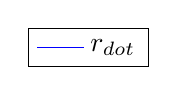
\begin{tikzpicture}

\begin{axis}[%
width=\figurewidth,
height=\figureheight,
scale only axis,
xmin=0,
xmax=30,
ymin=-0.15,
ymax=0.25,
axis x line*=bottom,
axis y line*=left,
legend style={at={(0.03,0.97)},anchor=north west,draw=black,fill=white,legend cell align=left}
]
\addplot [color=blue,solid]
  table[row sep=crcr]{0	-1.62384530621676e-08\\
0.1	-1.62384530621676e-08\\
0.2	-8.77999054483983e-09\\
0.3	-2.77340294402761e-09\\
0.4	1.53393641073239e-09\\
0.5	4.39613583758808e-09\\
0.6	6.07595533478803e-09\\
0.7	6.81537037334432e-09\\
0.8	6.83324467112324e-09\\
0.9	6.32431537600687e-09\\
1	5.45838320802251e-09\\
1.1	4.37992238175788e-09\\
1.2	3.20826860880001e-09\\
1.3	2.03843709598549e-09\\
1.4	9.42541666006244e-10\\
1.5	-2.8268300264337e-11\\
1.6	-8.41469565325494e-10\\
1.7	-1.48055715986349e-09\\
1.8	-1.94230060909849e-09\\
1.9	-2.23398962723224e-09\\
2	-2.37077934000173e-09\\
2.1	-2.37322536184817e-09\\
2.2	-2.26507740698939e-09\\
2.3	-2.0713778306727e-09\\
2.4	-1.8168906674033e-09\\
2.5	-1.52486773274068e-09\\
2.6	-1.21614231273599e-09\\
2.7	-9.08527983531013e-10\\
2.8	-6.16490497858796e-10\\
2.9	-3.51054085527178e-10\\
3	-1.19900136877121e-10\\
3.1	7.23848073697748e-11\\
3.2	2.23953505845936e-10\\
3.3	3.35273704544397e-10\\
3.4	4.0866961849756e-10\\
3.5	4.47858638981955e-10\\
3.6	4.57507232849729e-10\\
3.7	4.42824385714607e-10\\
3.8	4.09205487013732e-10\\
3.9	3.61934645218254e-10\\
4	3.05948895117948e-10\\
4.1	2.45664170538291e-10\\
4.2	1.84859747179452e-10\\
4.3	1.26615749602868e-10\\
4.4	7.32966429046957e-11\\
4.5	2.657276921967e-11\\
4.6	-1.25283736699842e-11\\
4.7	-4.35492531454334e-11\\
4.8	-6.65155753013739e-11\\
4.9	-8.18424972026189e-11\\
5	-9.02397778287304e-11\\
5.1	-9.26206703699564e-11\\
5.2	-9.0018289602479e-11\\
5.3	-8.35121241027337e-11\\
5.4	-7.41663357857751e-11\\
5.5	-6.29806227786175e-11\\
5.6	-5.08536188555337e-11\\
5.7	-3.85582511828585e-11\\
5.8	-2.67279540242926e-11\\
5.9	-1.58523504652924e-11\\
6	-6.28078765754249e-12\\
6.1	1.7679432746877e-12\\
6.2	8.19134420259856e-12\\
6.3	1.29859952814875e-11\\
6.4	1.62287922968293e-11\\
6.5	1.80578227406401e-11\\
6.6	1.86539195616326e-11\\
6.7	1.82236444223839e-11\\
6.8	1.69842676435526e-11\\
6.9	1.51510971398649e-11\\
7	1.29273147972419e-11\\
7.1	1.04963694325306e-11\\
7.2	8.01676713430228e-12\\
7.3	5.61908974075964e-12\\
7.4	3.40494971627636e-12\\
7.5	1.44755501395267e-12\\
7.6	-2.06436911564644e-13\\
7.7	-1.53413265028884e-12\\
7.8	-2.53297277358518e-12\\
7.9	-3.21697146189476e-12\\
8	-3.61286407014145e-12\\
8.1	-3.75636553248205e-12\\
8.2	-3.68870830825792e-12\\
8.3	-3.45356609385587e-12\\
8.4	-3.09446283701387e-12\\
8.5	-2.65265972843086e-12\\
8.6	-2.16557574959442e-12\\
8.7	-1.66568970124065e-12\\
8.8	-1.17990025302189e-12\\
8.9	-7.29272436710005e-13\\
9	-3.29123989346869e-13\\
9.1	1.06231822926024e-14\\
9.2	2.84899850293372e-13\\
9.3	4.9280778026059e-13\\
9.4	6.36864902990846e-13\\
9.5	7.22231248331123e-13\\
9.6	7.55953703497972e-13\\
9.7	7.46253841327985e-13\\
9.8	7.01910765296167e-13\\
9.9	6.31713336697072e-13\\
10	5.44036387120639e-13\\
10.0137604070044	4.46514929251882e-13\\
10.0275208140088	4.46514929251882e-13\\
10.1	4.46514929251882e-13\\
10.1094087443329	-0.0459963732635423\\
10.1188174886658	-0.0459963732635423\\
10.1658612103304	-0.0459963732635423\\
10.2	-0.0459963732635423\\
10.3	-0.0768914608849033\\
10.4	-0.0955172819905193\\
10.5	-0.102393283575401\\
10.6	-0.101230333008197\\
10.7	-0.0941860304658525\\
10.8	-0.0809925572535441\\
10.9	-0.0641017638709199\\
11	-0.0456853909885805\\
11.1	-0.0274423626196791\\
11.2	-0.0106372594628397\\
11.3	0.00388380913954456\\
11.4	0.0156284249226547\\
11.5	0.0244065692088312\\
11.6	0.0293335593033009\\
11.7	0.0316900210478532\\
11.8	0.032247417194989\\
11.9	0.0313180321591271\\
12	0.0291898538094346\\
12.1	0.0261603866054108\\
12.2	0.0225221925885715\\
12.3	0.0185481893139573\\
12.4	0.0144805392781305\\
12.5	0.0105235216351973\\
12.6	0.0068398888387563\\
12.7	0.00355015917174622\\
12.8	0.000734270313910459\\
12.9	-0.0015649755724084\\
13	-0.00333721488313281\\
13.1	-0.00459906476544667\\
13.2	-0.00538833369961981\\
13.3	-0.00575825995224994\\
13.4	-0.00577206433583881\\
13.5	-0.00549798892417033\\
13.6	-0.00500523625053534\\
13.7	-0.00436018261285191\\
13.8	-0.00362388670188028\\
13.9	-0.00285010773392317\\
14	-0.00208409065369697\\
14.1	-0.00136199708321915\\
14.2	-0.00071088553231631\\
14.3	-0.000149137734372852\\
14.4	0.000312774288539612\\
14.5	0.000671282566497709\\
14.6	0.000928573366688289\\
14.7	0.00109137675357646\\
14.8	0.00116976610852598\\
14.9	0.00117598378391948\\
15	0.00112359561796015\\
15.1	0.00102630797641512\\
15.2	0.000897451211468372\\
15.3	0.000749356123573013\\
15.4	0.000592938864404923\\
15.5	0.000437436941535186\\
15.6	0.000290278030968276\\
15.7	0.000157062464338589\\
15.8	4.16384913281962e-05\\
15.9	-5.37511125805547e-05\\
16	-0.00012827191212566\\
16.1	-0.000182269460112191\\
16.2	-0.000217026869181893\\
16.3	-0.000234522859694632\\
16.4	-0.000237202029715839\\
16.5	-0.00022776624912972\\
16.6	-0.000208993344365956\\
16.7	-0.000183586726191248\\
16.8	-0.000154057401023628\\
16.9	-0.000122637946708833\\
17	-9.12265501943422e-05\\
17.1	-6.13580977388611e-05\\
17.2	-3.41985602872689e-05\\
17.3	-1.05584954646405e-05\\
17.4	9.07864865354387e-06\\
17.5	2.45176419576781e-05\\
17.6	3.58059191833052e-05\\
17.7	4.31848667695342e-05\\
17.8	4.70409363820348e-05\\
17.9	4.78590092875966e-05\\
18	4.61798622462584e-05\\
18.1	4.25630311508716e-05\\
18.2	3.75558568610102e-05\\
18.3	3.16690453092617e-05\\
18.4	2.53586918673251e-05\\
18.5	1.90144133441562e-05\\
18.6	1.29530004524357e-05\\
18.7	7.41684579993543e-06\\
18.8	2.57631133298375e-06\\
18.9	-1.46483371279034e-06\\
19	-4.66175733462598e-06\\
19.1	-7.01949013976312e-06\\
19.2	-8.58314673426591e-06\\
19.3	-9.42805600518595e-06\\
19.4	-9.65030043294669e-06\\
19.5	-9.35804899131549e-06\\
19.6	-8.6639558254956e-06\\
19.7	-7.67879274758089e-06\\
19.8	-6.50639112425384e-06\\
19.9	-5.23989021151539e-06\\
19.9605807921388	-3.95922569668483e-06\\
19.9893482375409	-3.95922569668483e-06\\
20	-3.95922569668483e-06\\
20.0100988555802	0.000610700271487986\\
20.0264373103001	0.000610700271487986\\
20.1	0.000610700271487986\\
20.2	0.0931808581952406\\
20.3	0.158397995669645\\
20.4	0.194476402284566\\
20.5	0.207936274971073\\
20.6	0.208502969541613\\
20.7	0.190914455420385\\
20.8	0.162111596256063\\
20.9	0.126689460576675\\
21	0.0888330758199891\\
21.1	0.0518360895644502\\
21.2	0.0181048574336308\\
21.3	-0.0107768512472129\\
21.4	-0.0339675093613029\\
21.5	-0.0512072690779094\\
21.6	-0.0619723780607132\\
21.7	-0.067282184080214\\
21.8	-0.0664783975666516\\
21.9	-0.0629762469169243\\
22	-0.0575182826981594\\
22.1	-0.05063337294588\\
22.2	-0.0428553071771593\\
22.3	-0.0346729678643615\\
22.4	-0.0265161680008385\\
22.5	-0.018742262494549\\
22.6	-0.0116297263747689\\
22.7	-0.00537933265729399\\
22.8	-0.000115016031486655\\
22.9	0.00410693973683599\\
23	0.00728915908684063\\
23.1	0.00948230827744911\\
23.2	0.0107741022600648\\
23.3	0.0112782538273264\\
23.4	0.0111240316868222\\
23.5	0.0104472727028517\\
23.6	0.00938229265167026\\
23.7	0.00805621145149418\\
23.8	0.00658463055397835\\
23.9	0.00506825240858275\\
24	0.00359079044281895\\
24.1	0.00221802396495185\\
24.2	0.000997901696666077\\
24.3	-3.84448347409134e-05\\
24.4	-0.000875072107615712\\
24.5	-0.00150902141681225\\
24.6	-0.00194793287423222\\
24.7	-0.00220760640608442\\
24.8	-0.00230962887914228\\
24.9	-0.00227918447309599\\
25	-0.00214311976954381\\
25.1	-0.00192828503698279\\
25.2	-0.00166029059630663\\
25.3	-0.00136241551495775\\
25.4	-0.00105493816221168\\
25.5	-0.000754726984992253\\
25.6	-0.000475069338133391\\
25.7	-0.000225707292321081\\
25.8	-1.30394881449996e-05\\
25.9	0.000159552479259738\\
26	0.000291292897296584\\
26.1	0.000383552280745964\\
26.2	0.000439379541415215\\
26.3	0.000462999804883825\\
26.4	0.000459418529579286\\
26.5	0.000434016505404814\\
26.6	0.000392213689540977\\
26.7	0.000339196354698104\\
26.8	0.000279708634314043\\
26.9	0.000217901948115413\\
27	0.000157248165338168\\
27.1	0.000100498124717308\\
27.2	4.96849266332111e-05\\
27.3	6.16166706918328e-06\\
27.4	-2.93347144270765e-05\\
27.5	-5.66015986568993e-05\\
27.6	-7.58783239917459e-05\\
27.7	-8.77498461486097e-05\\
27.8	-9.30519089615288e-05\\
27.9	-9.27820870735783e-05\\
28	-8.8019936237469e-05\\
28.1	-7.98584191273262e-05\\
28.2	-6.93478058377204e-05\\
28.3	-5.74524069686919e-05\\
28.4	-4.50198001109403e-05\\
28.5	-3.27616638874006e-05\\
28.6	-2.12449353132018e-05\\
28.7	-1.0891747039253e-05\\
28.8	-1.98646695238468e-06\\
28.9	5.31186376935859e-06\\
29	1.09533361141152e-05\\
29.1	1.49787338062309e-05\\
29.2	1.75001812572456e-05\\
29.3	1.86820009862808e-05\\
29.4	1.87226777098553e-05\\
29.5	1.78386005236959e-05\\
29.6	1.62500391206317e-05\\
29.7	1.41696133872613e-05\\
29.8	1.17933440244974e-05\\
29.9	9.29422864341797e-06\\
29.9695899823905	6.81817475345781e-06\\
30	6.81817475345781e-06\\
};
\addlegendentry{$r_{dot}$};

\end{axis}
\end{tikzpicture}%
	\end{center}
	\caption{Input: steering angle.}
	\label{fig:invariant}
\end{figure}

\end{document}